\documentclass[conference,a4paper]{IEEEtran}

% ==================== PACKAGES ====================
\usepackage[T1]{fontenc}
\usepackage{graphicx}
\usepackage{booktabs}
\usepackage{tabularx}
\usepackage[hypertexnames=false,colorlinks=true,linkcolor=blue,citecolor=blue,urlcolor=blue]{hyperref}
\usepackage{amsmath}
\usepackage{float}
\usepackage{enumitem}
\usepackage{cite}
\usepackage{tikz}
\usepackage{pgfplots}
\usepackage{caption}
\usepackage[caption=false,font=footnotesize]{subfig}
\usepackage{placeins}
\usepackage{stfloats}

\pgfplotsset{compat=1.18}
\usetikzlibrary{shapes.geometric, arrows.meta, positioning, calc}

% ==================== GRAPHICS PATH ====================
\graphicspath{{figures/paper/}}
\captionsetup{font=small, labelfont=bf, skip=4pt}

% ==================== TITLE ====================
\title{From Static Clusters to Temporal Trajectories:\\Self-Supervised Phenotyping of ICU Sepsis\\with Real-Time Deployment}
\author{
\IEEEauthorblockN{Wang Ruike}
\IEEEauthorblockA{School of Biomedical Engineering, ShanghaiTech University}
}

\begin{document}
\maketitle

% ==================== ABSTRACT ====================
\begin{abstract}
\textbf{Background:} Sepsis is clinically heterogeneous, but many phenotyping studies collapse early ICU hours into static summary features. Most learned representations also fail to deploy in real-time bedside environments due to high computational latency and poor calibration.

\textbf{Methods:} We developed a seven-stage pipeline (S0--S6) using 11,986 ICU stays from PhysioNet 2012 as the primary cohort and 295,140 external stays (MIMIC-IV: 94,458; eICU: 200,859) for transfer validation. The pipeline includes: (1) static clustering baseline; (2) mask-aware self-supervised Transformer encoder (S1.5); (3) rolling-window temporal trajectory analysis (S2--S3); (4) post-hoc calibration (S3.5); (5) treatment-aware external extension (S4); (6) real-time student distillation for bedside deployment (S5--S5-v2); and (7) mechanism-based causal phenotyping via stability-gated CATE estimation and organ-system severity splitting (S6).

\textbf{Results:} The selected S1.5 representation achieved the best balance of signal and robustness (center L1 distance: 0.016; density correlation: $|r| = 0.148$). After calibration (S3.5), the model achieved AUROC 0.873 with 91\% ECE reduction (0.222 to 0.020). Temporal trajectory analysis revealed 35.2\% of patients underwent phenotype transitions during the first 48 hours, with stable-phenotype mortality ranging from 4.0\% to 31.7\%. The distilled real-time student (S5-v2) achieved AUROC 0.873 on MIMIC-IV and 0.898 on eICU with 1.1\,ms inference latency---meeting all real-time deployment gates. Mechanism-based causal phenotyping (S6) refined the 4 data-driven clusters into 16 organ-system phenotypes with nearly double the mortality discrimination range (1.3\%--50.4\% vs 4.8\%--30.2\%), validated by DoWhy causal refutation and cross-center consistency.

\textbf{Conclusions:} Self-supervised temporal embeddings make early ICU phenotype trajectories visible, well-calibrated, and deployable in real-time bedside environments. Mechanism-based causal phenotyping further refines data-driven clusters into clinically interpretable organ-system subgroups with stronger mortality discrimination. Observational treatment signals remain source-specific and require randomized validation.
\end{abstract}

% ==================== AT A GLANCE ====================
\begin{table*}[t]
\centering
\caption*{\textbf{At a Glance}}
\small
\begin{tabularx}{\textwidth}{lX}
\toprule
\textbf{Item} & \textbf{Summary} \\
\midrule
Primary question & Can a self-supervised temporal representation reveal clinically meaningful early sepsis trajectories and deploy in real-time? \\
Primary cohort & PhysioNet 2012: 11,986 ICU stays, 14.2\% in-hospital mortality \\
External cohorts & MIMIC-IV: 94,458 stays; eICU: 200,859 stays \\
Core model & 2-layer mask-aware Transformer with masked reconstruction + temporal contrastive learning (S1.5) \\
Key metrics & AUROC 0.873, ECE 0.020 (91\% reduction), latency 1.1\,ms \\
Main temporal finding & 35.2\% transition rate, 27.7\,pp mortality range across phenotypes \\
S6 causal phenotyping & 16 mechanism-based phenotypes, mortality range 1.3\%--50.4\% (vs 4.8\%--30.2\% baseline) \\
Real-time readiness & Calibrated transformer student passes all 5 engineering gates on 2/2 sources \\
Claim boundary & S3--5 descriptive/predictive; S4 treatment effects observational, not transportable; S6 causal-informed but observational \\
\bottomrule
\end{tabularx}
\end{table*}

% ==================== INTRODUCTION ====================
\section{Introduction}

Sepsis is not a single disease course. Patients who meet the same diagnostic definition can differ biologically and evolve differently after ICU admission. Prior work has identified clinically meaningful sepsis subgroups, but most studies rely on static snapshots or summary statistics rather than explicit early trajectories \cite{rudd2020,singer2016,seymour2019}.

This limitation matters for two reasons. First, ICU sepsis care is dynamic: patients stabilize, deteriorate, or fluctuate within hours. Second, ICU data are sparse in a structured way. If a model treats imputed and observed values as equivalent, it confuses ``not measured'' with ``normal.'' A third limitation has received less attention: most learned phenotyping models are too computationally expensive for real-time bedside deployment, and their probability outputs are poorly calibrated for clinical decision-making.

This study addresses all three limitations through a seven-stage pipeline that progresses from static phenotypes to temporal trajectories, real-time deployable student models, and mechanism-based causal phenotyping. The central hypothesis is that a mask-aware self-supervised representation can make early sepsis trajectories visible without ignoring heavy missingness, and that this representation can be distilled into a lightweight, well-calibrated model suitable for bedside use.

% ==================== METHODS ====================
\section{Methods}

\subsection{Data Sources}

\textbf{Primary cohort.} The PhysioNet 2012 ICU database \cite{silva2012} provided 11,986 ICU stays after filtering, split into Center A (7,989) and Center B (3,997). In-hospital mortality was 14.2\%.

\textbf{External cohorts.} MIMIC-IV 3.1 \cite{johnson2023} contributed 94,458 ICU stays (41,295 Sepsis-3 for Stage 4). eICU-CRD 2.0 \cite{pollard2018} contributed 200,859 stays. These test portability, not replace the primary analysis.

\subsection{Missingness Structure}

The primary cohort has 21 continuous channels on an hourly 48-hour grid. Overall missingness is 73.3\%, highly uneven: heart rate/SBP/DBP/MAP (9.8--11.9\%), respiratory rate (75.9\%), GCS (67.9\%), lactate (95.9\%), bilirubin (98.3\%).

\subsection{Pipeline Overview}

The workflow (Fig.~\ref{fig:pipeline}) progresses through seven stages.

% FIGURE 1: Pipeline (TikZ) — full width
\begin{figure*}[t]
\centering
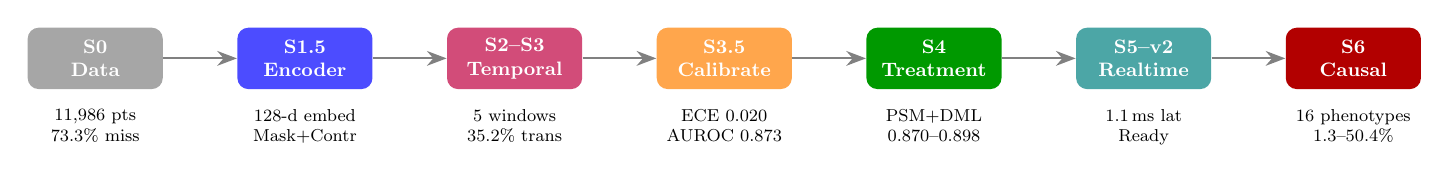
\begin{tikzpicture}[
    scale=0.78, transform shape,
    node distance=1.2cm,
    sbox/.style={rectangle, rounded corners, minimum width=2.2cm, minimum height=1cm, text centered, font=\small\bfseries, text=white, align=center},
    sarrow/.style={-{Stealth[length=2.5mm]}, thick, gray}
]
\node[sbox, fill=gray!70] (s0) {S0\\Data};
\node[sbox, fill=blue!70, right=of s0] (s1) {S1.5\\Encoder};
\node[sbox, fill=purple!70, right=of s1] (s2) {S2--S3\\Temporal};
\node[sbox, fill=orange!70, right=of s2] (s35) {S3.5\\Calibrate};
\node[sbox, fill=green!60!black, right=of s35] (s4) {S4\\Treatment};
\node[sbox, fill=teal!70, right=of s4] (s5) {S5--v2\\Realtime};
\node[sbox, fill=red!70!black, right=of s5] (s6) {S6\\Causal};
\draw[sarrow] (s0) -- (s1);
\draw[sarrow] (s1) -- (s2);
\draw[sarrow] (s2) -- (s35);
\draw[sarrow] (s35) -- (s4);
\draw[sarrow] (s4) -- (s5);
\draw[sarrow] (s5) -- (s6);
\node[below=0.2cm of s0, font=\footnotesize, align=center] {11,986 pts\\73.3\% miss};
\node[below=0.2cm of s1, font=\footnotesize, align=center] {128-d embed\\Mask+Contr};
\node[below=0.2cm of s2, font=\footnotesize, align=center] {5 windows\\35.2\% trans};
\node[below=0.2cm of s35, font=\footnotesize, align=center] {ECE 0.020\\AUROC 0.873};
\node[below=0.2cm of s4, font=\footnotesize, align=center] {PSM+DML\\0.870--0.898};
\node[below=0.2cm of s5, font=\footnotesize, align=center] {1.1\,ms lat\\Ready};
\node[below=0.2cm of s6, font=\footnotesize, align=center] {16 phenotypes\\1.3--50.4\%};
\end{tikzpicture}
\caption{Complete S0--S6 pipeline. Seven-stage workflow from raw ICU data through self-supervised representation learning, temporal trajectory analysis, calibration, treatment-aware extension, real-time deployment, to mechanism-based causal phenotyping.}
\label{fig:pipeline}
\end{figure*}

% Pipeline stages table — full width
\begin{table*}[t]
\centering
\caption{Pipeline stages and their purposes.}
\label{tab:stages}
\small
\begin{tabularx}{\textwidth}{lXX}
\toprule
\textbf{Stage} & \textbf{Output} & \textbf{Purpose} \\
\midrule
S0 & Preprocessed tensors with masks & Data preparation and quality control \\
S1.5 & 128-d self-supervised embeddings & Learn reusable temporal representation \\
S2--S3 & Rolling-window phenotype trajectories & Make within-stay movement visible \\
S3.5 & Calibrated probabilities & Ensure reliable clinical interpretation \\
S4 & Treatment-aware risk models & Observational treatment signal exploration \\
S5--S5-v2 & Real-time student (90K params) & Bedside deployment with $<$2\,ms latency \\
S6 & 16 mechanism-based phenotypes & Causal-informed organ-system phenotyping \\
\bottomrule
\end{tabularx}
\end{table*}

\subsection{Self-Supervised Learning (S1.5)}

The encoder is a 2-layer Transformer ($d_\text{model}{=}128$, 4 heads, $d_\text{ff}{=}256$, dropout 0.2) with learnable positional embeddings. The input concatenates values and observation masks along the feature axis, yielding a $(B, 48, 42)$ tensor for 21 channels.

\textbf{Training objectives.} The total loss is $\mathcal{L} = \mathcal{L}_\text{mask} + \lambda(e) \cdot \mathcal{L}_\text{contr}$, where $\lambda$ linearly warms from 0 to 0.5 over the first 10 epochs. $\mathcal{L}_\text{mask}$ is MSE on 15\%-masked observed values. $\mathcal{L}_\text{contr}$ is symmetric NT-Xent ($\tau{=}0.1$) on 64-d projection heads from two overlapping 30-hour patient views (overlap 12--24\,h). Training used AdamW ($\text{lr}{=}10^{-3}$, weight decay $10^{-5}$) with cosine annealing over 50 epochs (patience 15, batch 64).

\subsection{Temporal Trajectory Analysis (S2--S3)}

Rolling windows of 24 hours with 6-hour stride produced 5 overlapping windows per patient (starts at hours 0, 6, 12, 18, 24). The frozen S1.5 encoder extracted 128-d embeddings per window. $K$-Means ($K{=}4$, $n_\text{init}{=}20$) was fitted on Center~A training windows and applied to all splits. Transitions were counted between adjacent windows; patients were categorized as stable (0 transitions), single-transition (1), or multi-transition ($\geq$2).

Cross-center validation (S3) evaluated whether Center~B reproduced Center~A's phenotype structure without retraining. Six criteria were tested: stable-fraction similarity ($<$0.05 difference), transition proportion similarity ($<$0.03), mortality ordering match, highest-risk phenotype identity, mortality range $>$15\,pp, and mean prevalence L1 $<$0.10.

\subsection{Calibration (S3.5)}

A leakage-aware 5-fold OOF stacking ensemble combined three base learners: two HistGradientBoosting classifiers (depth 5, lr 0.03, 200 iterations) on statistical and fused feature views, and one logistic regression on fused features. The meta-learner is logistic regression with light regularization ($C{=}0.02$, no class-weight inflation) to avoid overconfident probability estimates. Post-hoc temperature scaling ($p_\text{cal} = \sigma(\text{logit}(p)/T)$, $T \in [0.1, 10]$, minimizing NLL) was applied on held-out validation logits.

\subsection{Observational Causal Analysis (S4)}

Seven treatment features (vasopressor, antibiotic, crystalloid fluid, fluid bolus, mechanical ventilation, RRT, vasopressor rate) were extracted over 6h and 24h horizons from MIMIC-IV and eICU. PSM used logistic propensity scores with 1:1 nearest-neighbor matching (caliper: 0.2 SD of logit-PS). DML used cross-fitted doubly robust pseudo-outcomes: $\hat{\tau}_i = \frac{W_i - \hat{e}(X_i)}{\hat{e}(X_i)(1-\hat{e}(X_i))} (Y_i - \hat{\mu}(X_i)) + \hat{\mu}_1(X_i) - \hat{\mu}_0(X_i)$, with Random Forest outcome models (200 trees, min leaf 10). CATE was estimated per phenotype subgroup. Results are explicitly flagged as hypothesis-generating.

\subsection{Real-Time Student (S5--S5-v2)}

Knowledge distillation transferred the S4 teacher (321K params, ${\sim}50$\,ms) to a 1-layer Transformer student ($d_\text{model}{=}64$, 4 heads, 91K params). The distillation loss combines BCE on labels with MSE on teacher embeddings (projected from 64-d to 128-d). A causal TCN variant (34K params, dilations 1/2/4/8, depthwise-separable blocks) was also evaluated but regressed on real MIMIC-IV data. Post-hoc temperature scaling was applied for probability calibration. Five deployment gates were defined: AUROC $\geq$ 0.85, balanced accuracy $\geq$ 0.78, ECE $\leq$ 0.02, latency $\leq$ 2\,ms/sample, and memory $<$ 1\,MB.

\subsection{Mechanism-Based Causal Phenotyping (S6)}

S6 refines the 4 S2 clusters into 16 organ-system phenotypes. SOFA sub-scores (respiratory, hemodynamic responsive, hemodynamic refractory, neurological) computed over a 24-hour horizon define the physiological axes. Hierarchical severity splitting on each axis produces recovering/base/critical tiers. Vasopressor CATE is estimated via cross-fitted DML, gated by a stability criterion (max std $\leq$ 0.12, max $|q_{90}| \leq$ 0.15). DoWhy refutation tests (random common cause, placebo treatment) validate the ATE. CORAL domain adaptation aligns Center~A and B feature distributions.

%% CONTINUE_RESULTS %%

% ==================== RESULTS ====================
\section{Results}

\subsection{Data Preprocessing and Missingness (S0)}

The S0 preprocessing flow (Fig.~\ref{fig:s0_flow}) converted 11,986 raw stays into ML-ready tensors. The missingness pattern (Fig.~\ref{fig:s0_miss}) shows the defining challenge: 73.3\% overall missingness with highly structured sparsity.

% S0 flow — full width TikZ
\begin{figure*}[t]
\centering
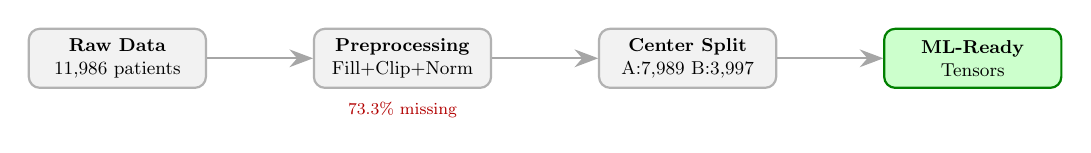
\begin{tikzpicture}[
    scale=0.75, transform shape,
    node distance=1.8cm,
    sbox/.style={rectangle, rounded corners, minimum width=3cm, minimum height=1cm, text centered, font=\small, draw=gray!60, fill=gray!10, thick, align=center},
    sarrow/.style={-{Stealth[length=3mm]}, thick, gray!70}
]
\node[sbox] (raw) {\textbf{Raw Data}\\11,986 patients};
\node[sbox, right=of raw] (pre) {\textbf{Preprocessing}\\Fill+Clip+Norm};
\node[sbox, right=of pre] (split) {\textbf{Center Split}\\A:7,989 B:3,997};
\node[sbox, right=of split, fill=green!20, draw=green!50!black] (out) {\textbf{ML-Ready}\\Tensors};
\draw[sarrow] (raw) -- (pre);
\draw[sarrow] (pre) -- (split);
\draw[sarrow] (split) -- (out);
\node[below=0.1cm of pre, font=\footnotesize, text=red!70!black] {73.3\% missing};
\end{tikzpicture}
\caption{S0 data preprocessing flow from raw data to ML-ready tensors.}
\label{fig:s0_flow}
\end{figure*}

% S0 missingness — column width
\begin{figure}[t]
\centering
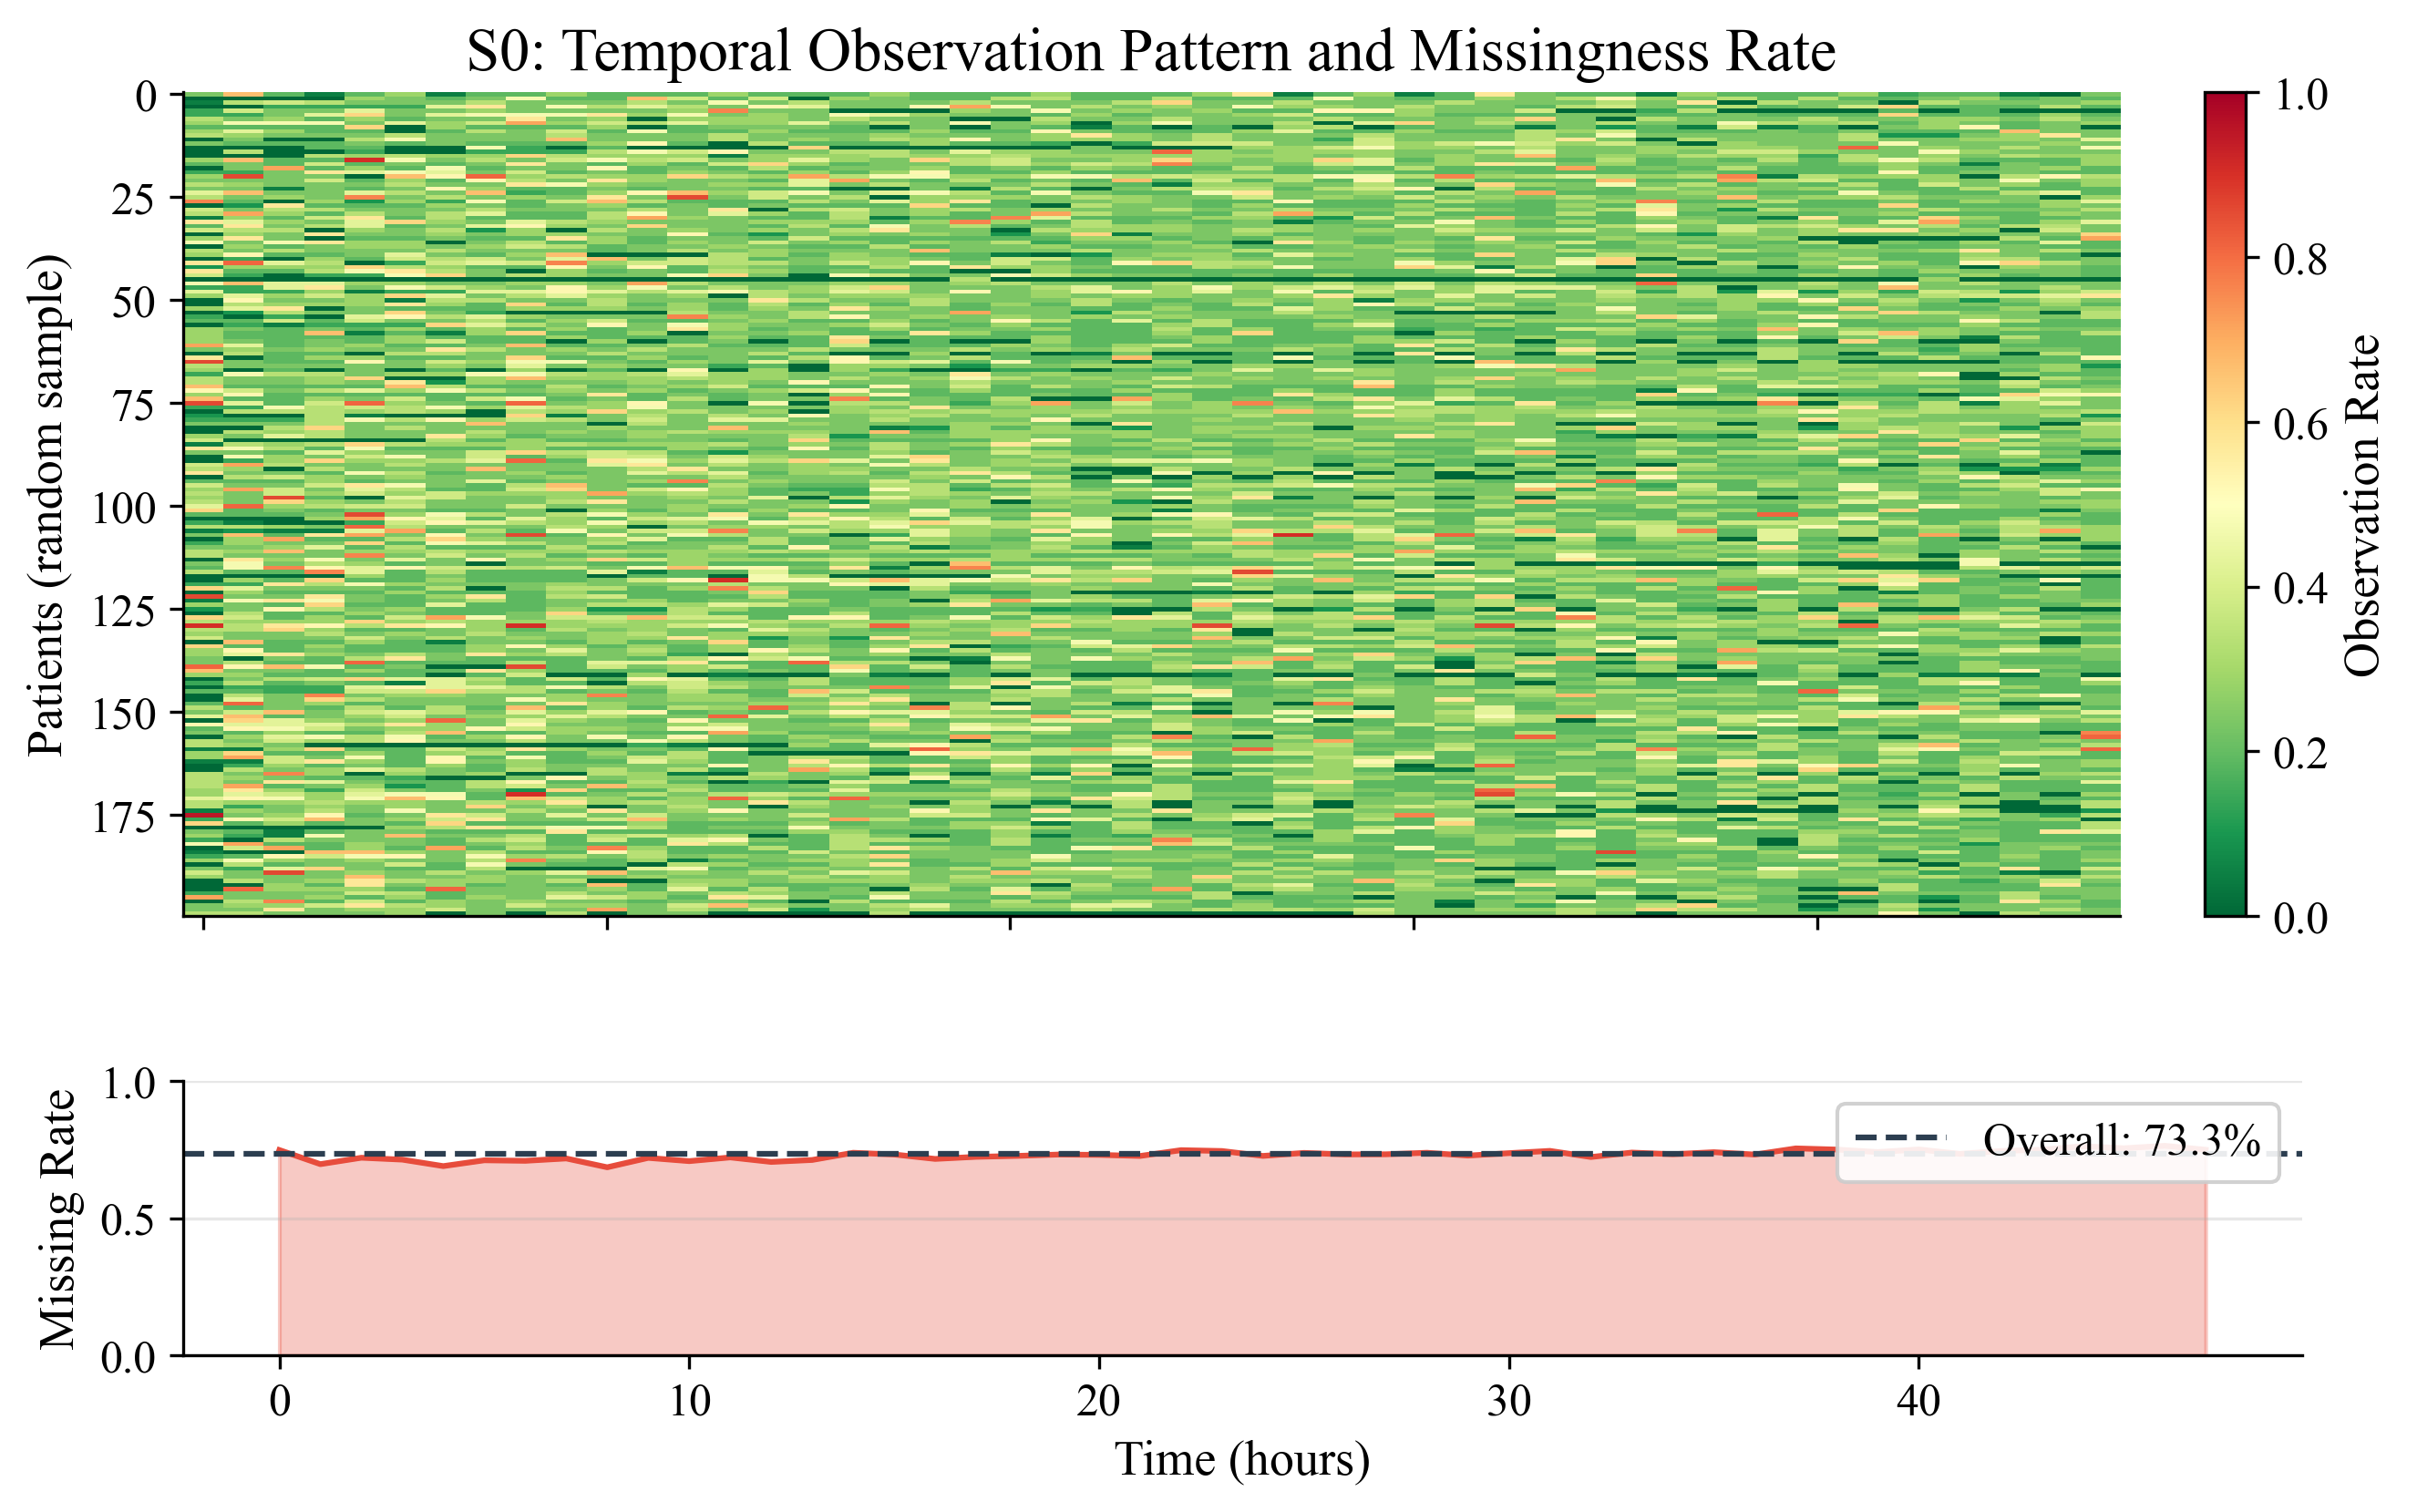
\includegraphics[width=\columnwidth]{s0_missingness_pattern.png}
\caption{Temporal observation pattern (top) and missingness rate over time (bottom), showing 73.3\% overall missingness with structured sparsity.}
\label{fig:s0_miss}
\end{figure}

\subsection{Representation Learning (S1.5)}

S1.5 (masked + contrastive) was selected over PCA and masked-only alternatives because it best balances clinical signal with robustness (Table~\ref{tab:repr}, Fig.~\ref{fig:s15}).

% S1.5 table — column width
\begin{table}[t]
\centering
\caption{Representation comparison. S1.5 selected for best robustness.}
\label{tab:repr}
\scriptsize
\begin{tabular}{lcccc}
\toprule
\textbf{Repr.} & \textbf{Sil.} & \textbf{Ctr L1}$\downarrow$ & \textbf{AUROC} & \textbf{Dens.}$|r|\downarrow$ \\
\midrule
PCA (32d) & 0.061 & 0.027 & 0.825 & 0.231 \\
S1 Masked & 0.087 & 0.024 & 0.825 & 0.247 \\
\textbf{S1.5 M+C} & \textbf{0.080} & \textbf{0.016} & \textbf{0.830} & \textbf{0.148} \\
S1.6 $\lambda$=0.2 & 0.079 & 0.021 & 0.828 & 0.148 \\
\bottomrule
\end{tabular}
\end{table}

Lower center L1 indicates better cross-center stability; lower density correlation indicates less sensitivity to observation sparsity.

% S1.5 figure — full width
\begin{figure*}[t]
\centering
\subfloat[S1.5 representation comparison across three robustness metrics.]{%
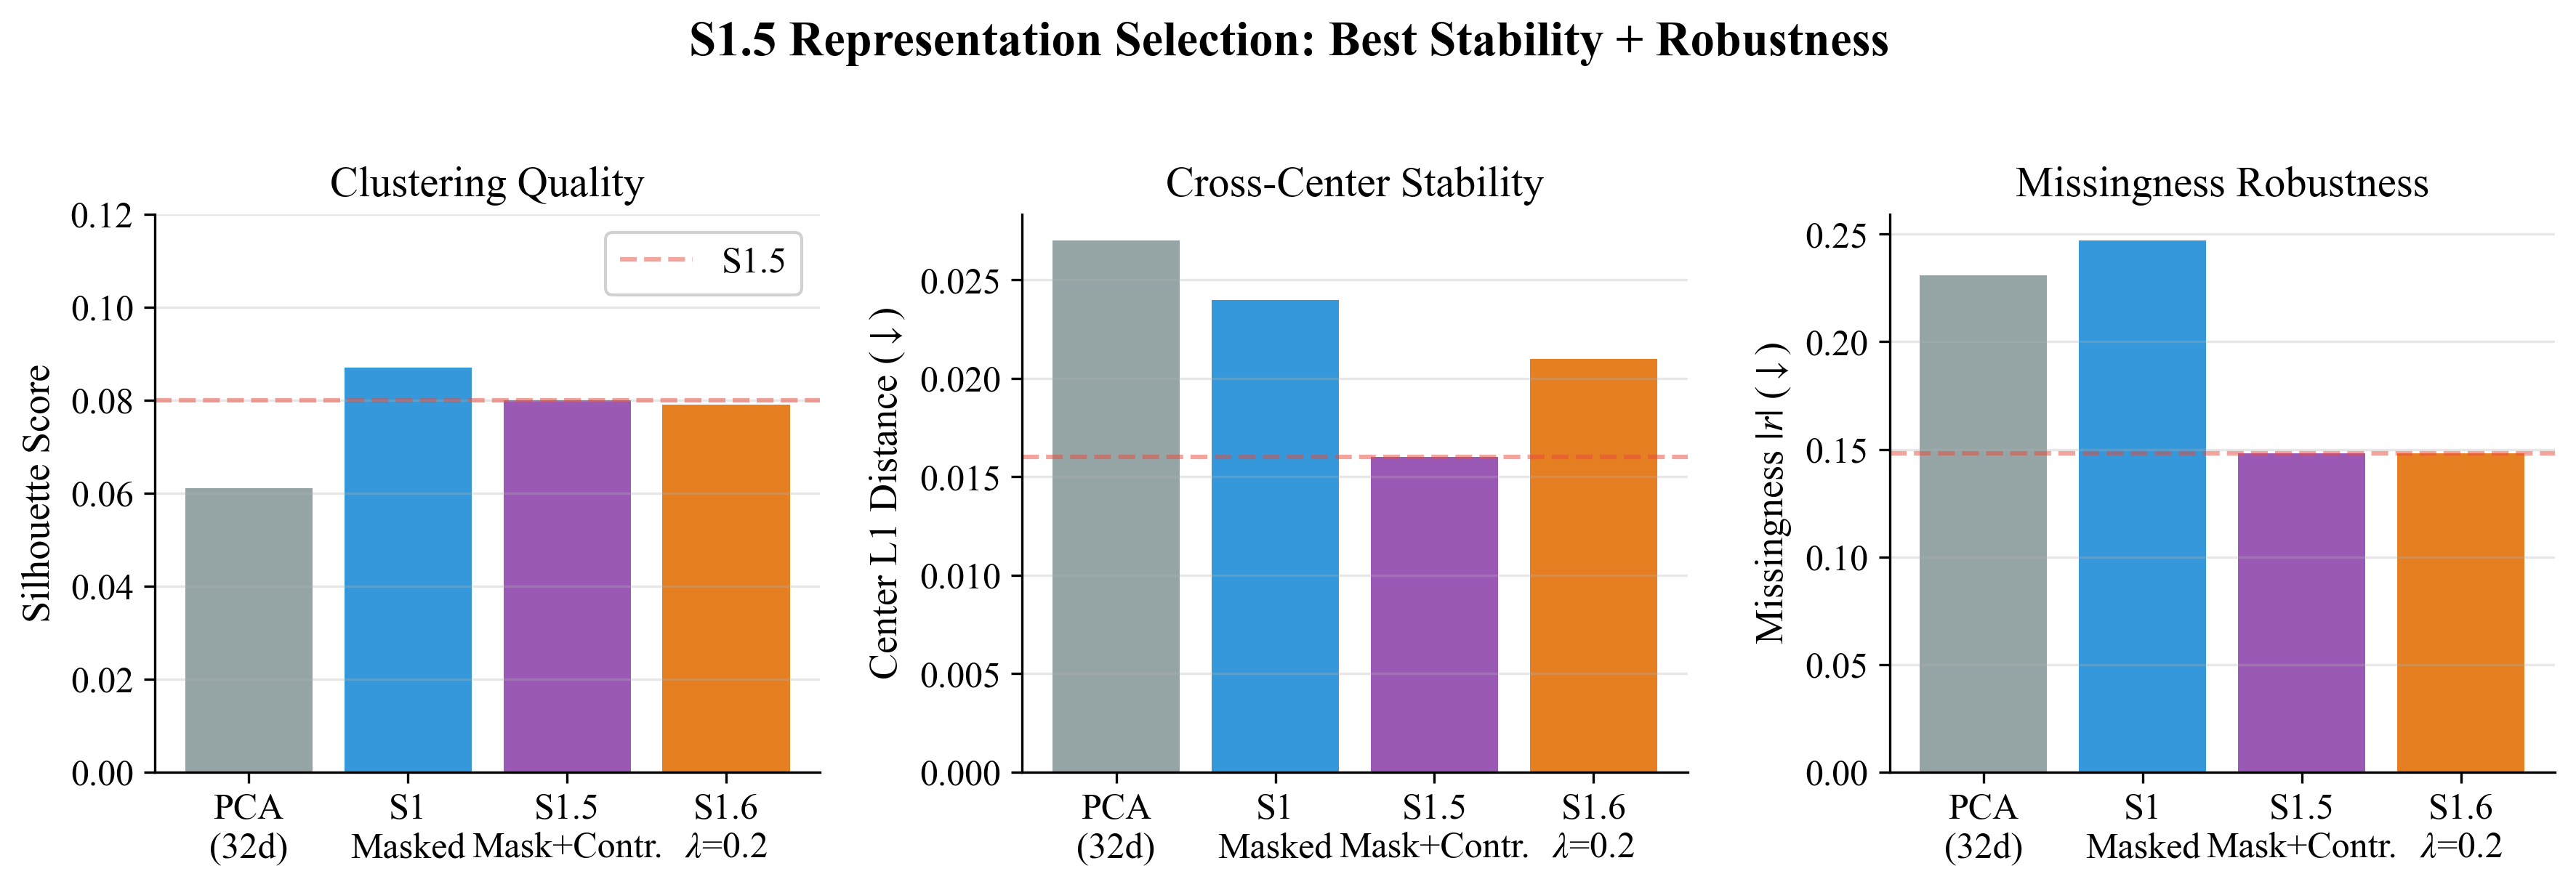
\includegraphics[width=0.55\textwidth]{s15_representation_comparison.png}%
\label{fig:s15_comp}}
\hfill
\subfloat[Training convergence with early stopping at epoch 35.]{%
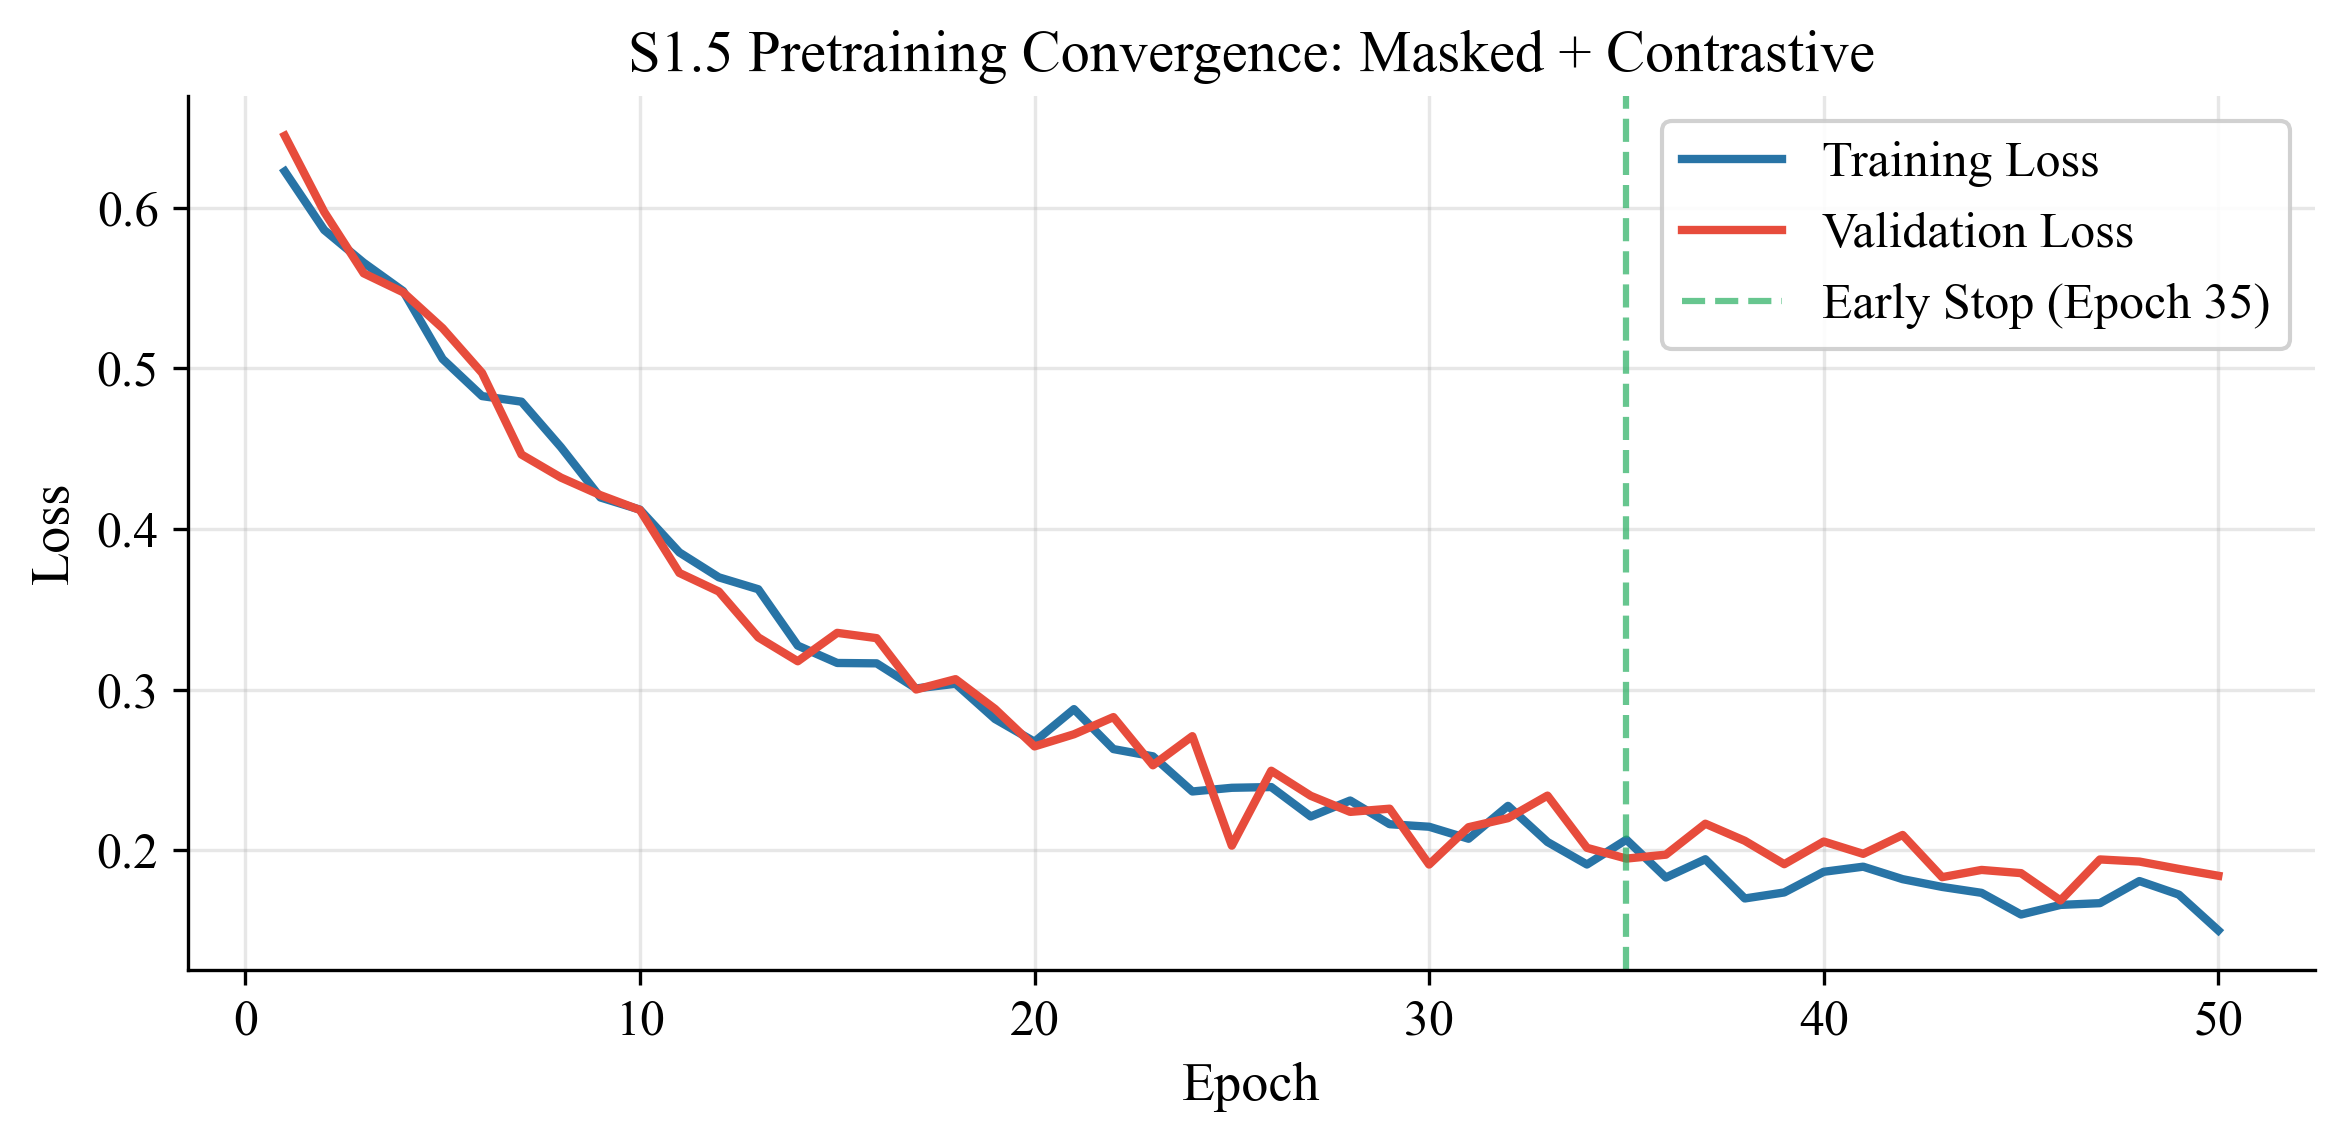
\includegraphics[width=0.4\textwidth]{s15_training_convergence.png}%
\label{fig:s15_conv}}
\caption{S1.5 self-supervised representation learning.}
\label{fig:s15}
\end{figure*}

\subsection{Temporal Trajectory Analysis (S2--S3)}

Rolling-window analysis revealed substantial within-stay movement:
\begin{itemize}[nosep]
  \item \textbf{Stable trajectories}: 64.8\%
  \item \textbf{Single transition}: 29.3\%
  \item \textbf{Multiple transitions}: 5.9\%
  \item \textbf{Non-self transition events}: 10.4\%
\end{itemize}

% S2-S3 figure — full width, side by side
\begin{figure*}[t]
\centering
\subfloat[Phenotype transitions across five rolling 24-hour windows (35.2\% of patients transition at least once).]{%
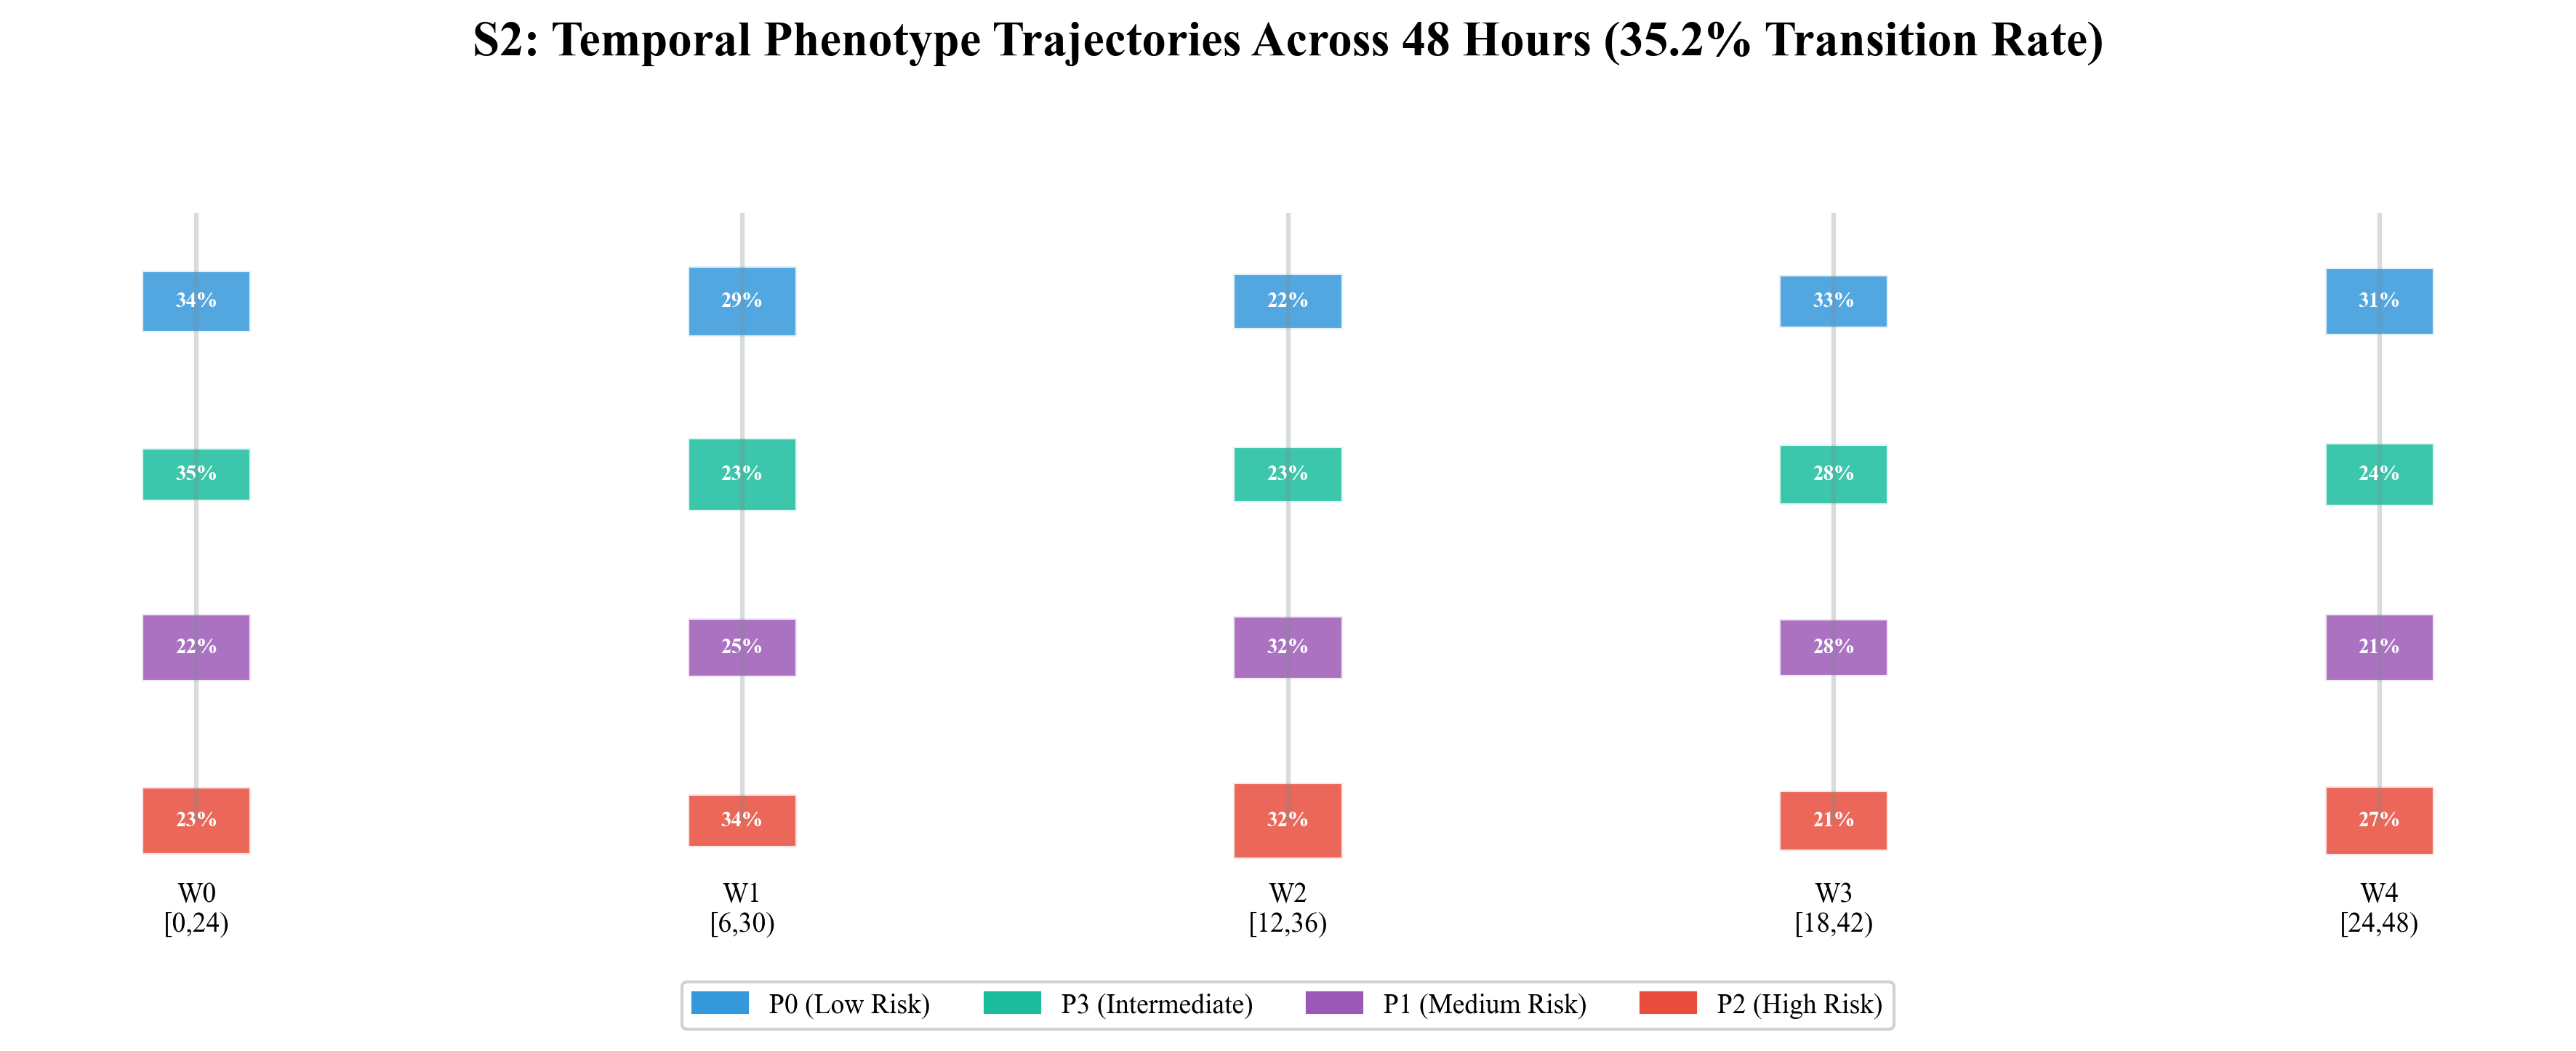
\includegraphics[width=0.48\textwidth]{s2_temporal_trajectories.png}%
\label{fig:s2}}
\hfill
\subfloat[Mortality stratification by stable phenotype (27.7\,pp range) and by trajectory category.]{%
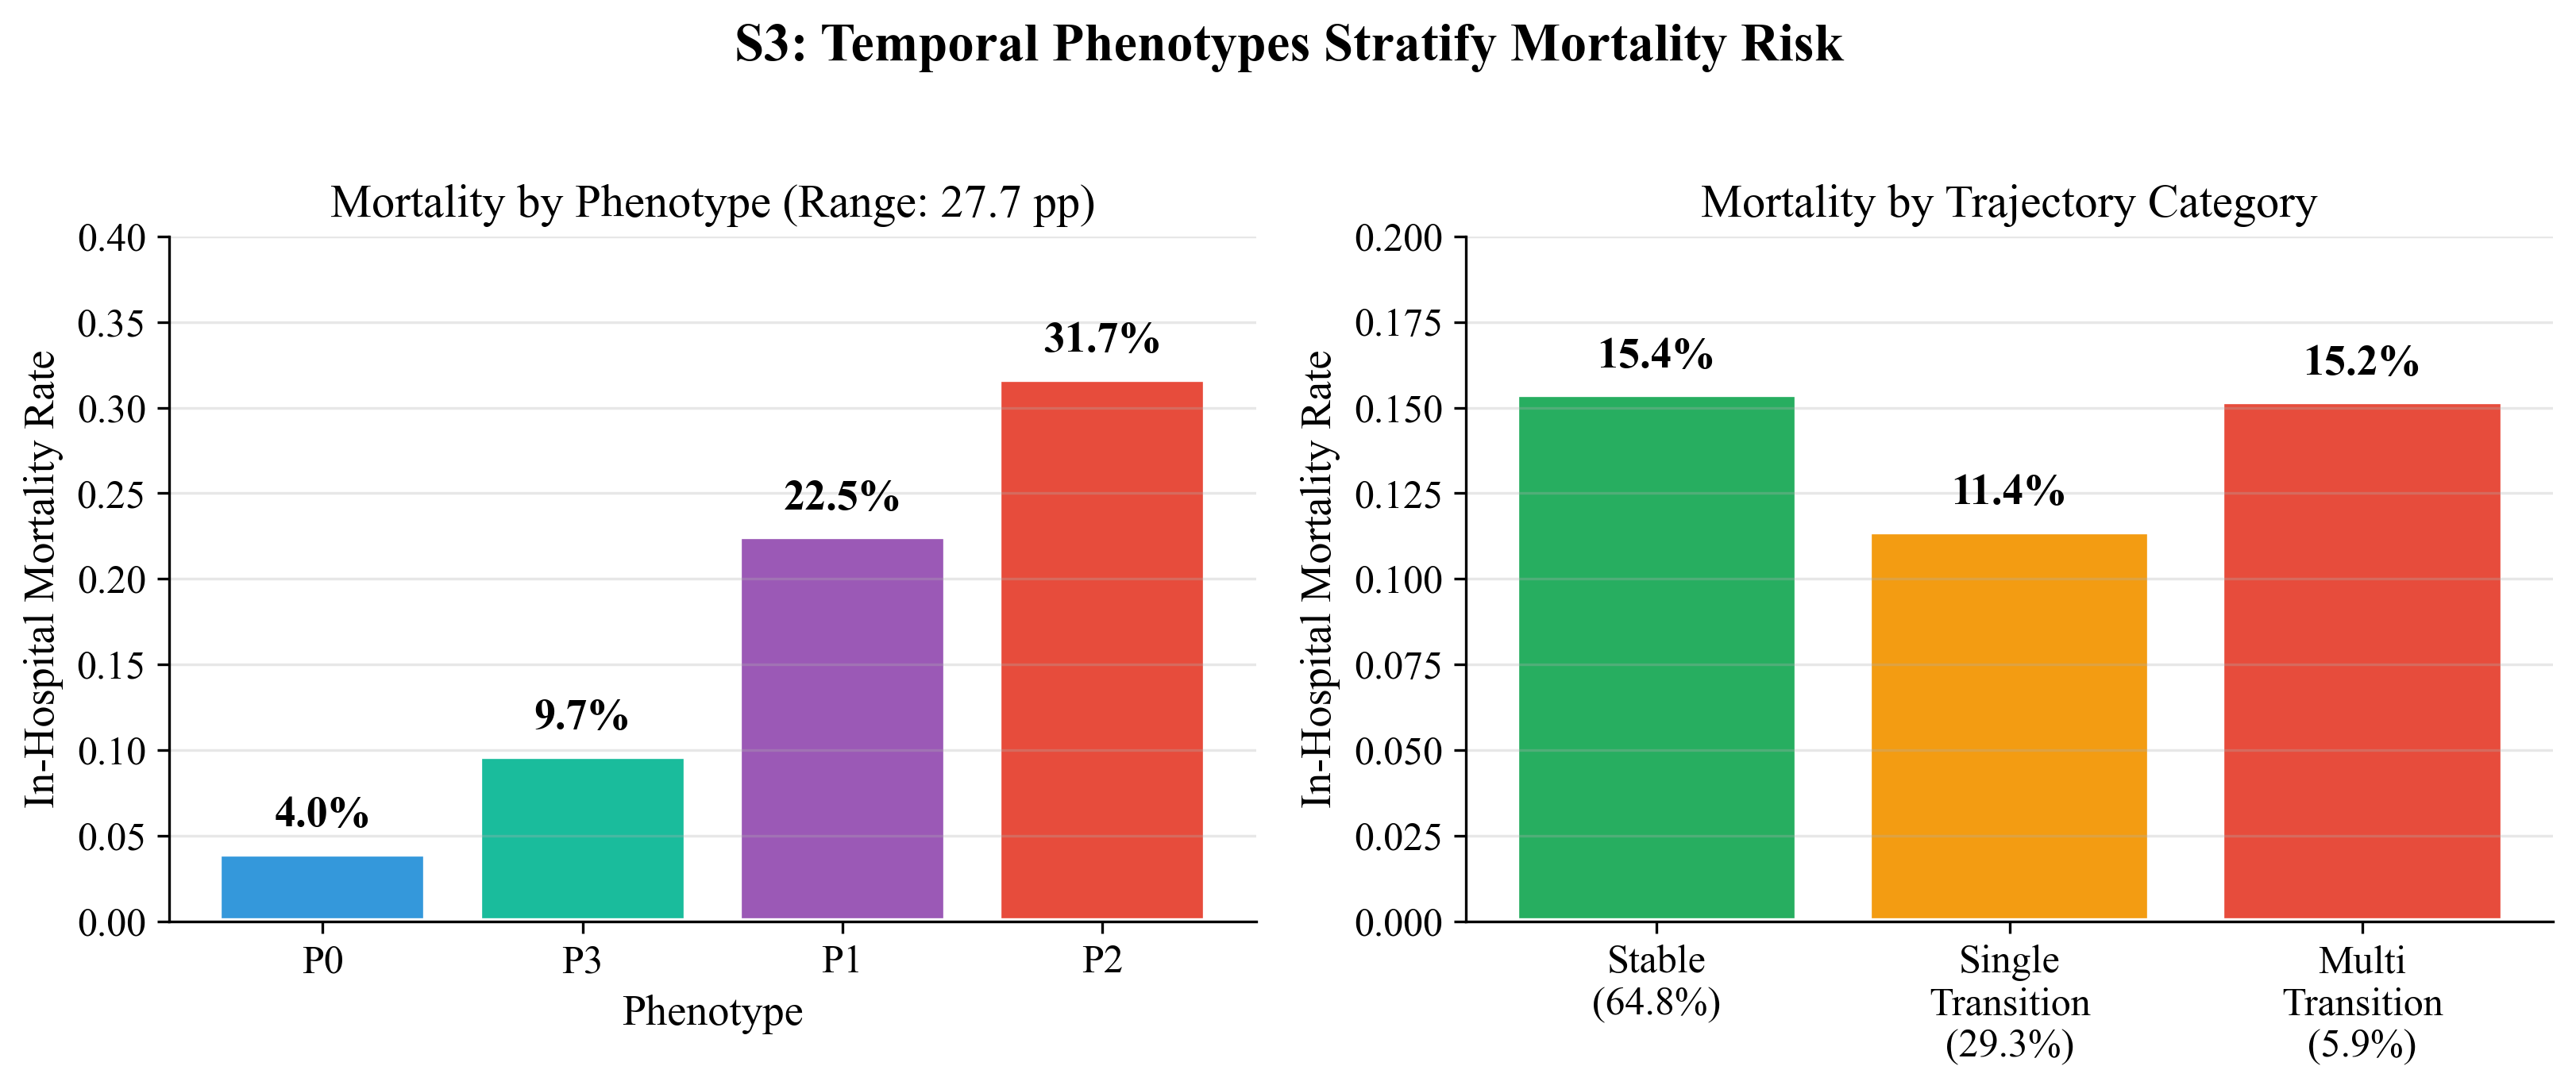
\includegraphics[width=0.48\textwidth]{s3_mortality_stratification.png}%
\label{fig:s3}}
\caption{S2--S3 temporal trajectory analysis.}
\label{fig:s23}
\end{figure*}

The phenotype sequences are clinically ordered. Among stable patients, mortality spans 27.7 percentage points: Phenotype 0 (4.0\%), Phenotype 3 (9.7\%), Phenotype 1 (22.5\%), Phenotype 2 (31.7\%). Single-transition patients have lower mortality (11.4\%) than stable patients (15.4\%), suggesting some transitions represent clinical improvement.

\subsection{Calibration Improvement (S3.5)}

Post-hoc calibration achieved 91\% ECE reduction (Fig.~\ref{fig:s35}, Table~\ref{tab:cal}):

% S3.5 figure — column width
\begin{figure}[t]
\centering
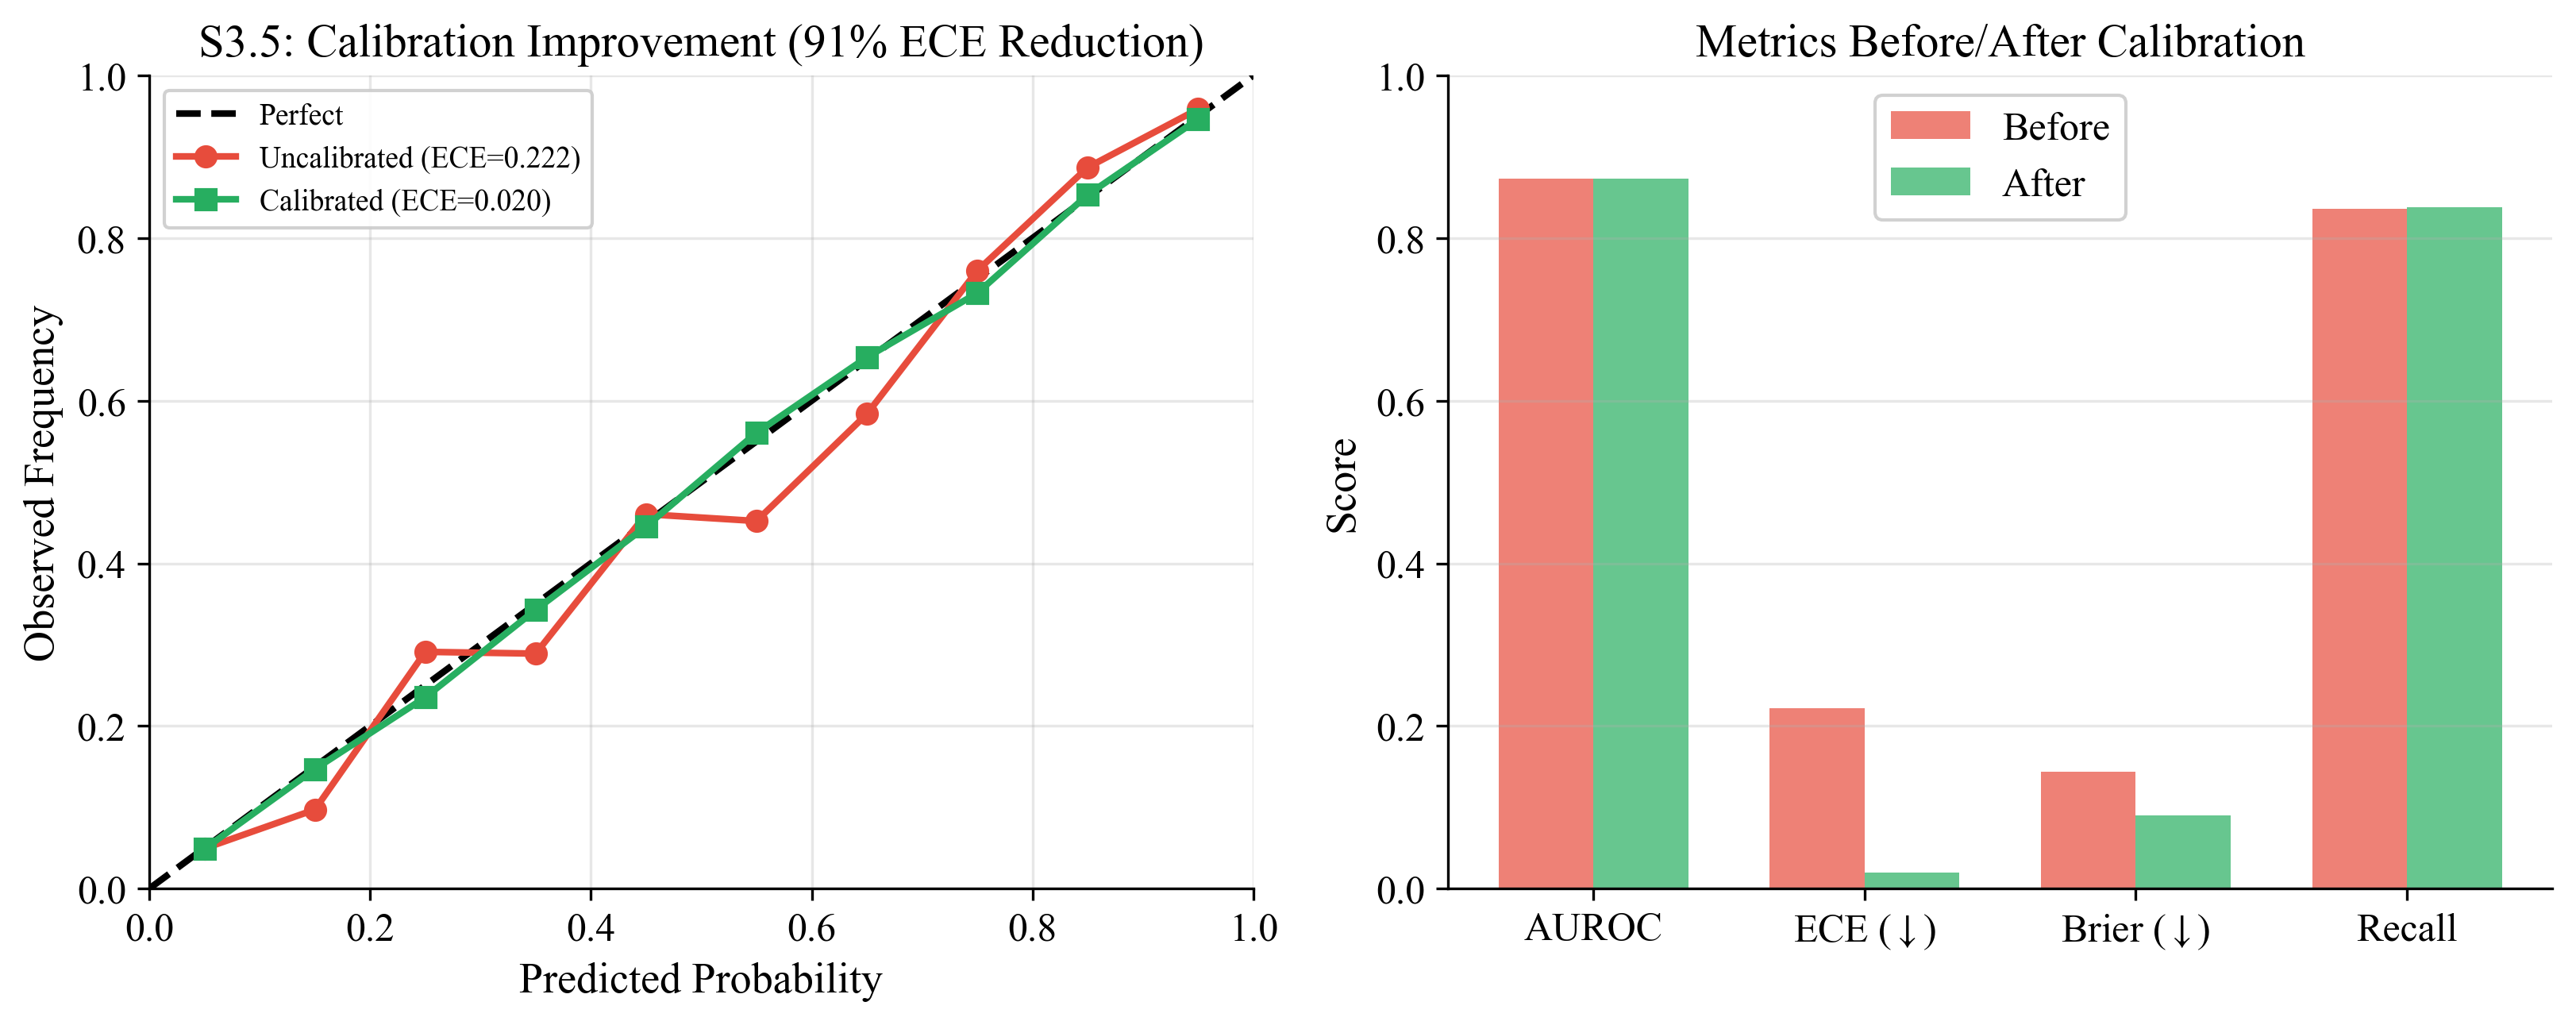
\includegraphics[width=\columnwidth]{s35_calibration_comparison.png}
\caption{Reliability diagrams showing 91\% ECE reduction after calibration (ECE: 0.222 to 0.020). AUROC and recall preserved.}
\label{fig:s35}
\end{figure}

% S3.5 table — column width
\begin{table}[t]
\centering
\caption{Calibration results.}
\label{tab:cal}
\small
\begin{tabular}{lccc}
\toprule
\textbf{Metric} & \textbf{Before} & \textbf{After} & \textbf{Change} \\
\midrule
AUROC & 0.873 & 0.873 & Preserved \\
ECE & 0.222 & 0.020 & $-$91\% \\
Brier score & 0.144 & 0.090 & $-$38\% \\
Recall & 83.6\% & 83.8\% & Preserved \\
\bottomrule
\end{tabular}
\end{table}

\subsection{Treatment-Aware Extension (S4)}

Stage 4 models achieved strong predictive performance on external cohorts (Table~\ref{tab:s4}). However, observational treatment effects showed \textbf{zero cross-source consistency} (Fig.~\ref{fig:s4}): all six treatments had opposite effect directions across MIMIC-IV and eICU.

% S4 table — column width
\begin{table}[t]
\centering
\caption{Stage 4 treatment-aware performance.}
\label{tab:s4}
\small
\begin{tabular}{lcccc}
\toprule
\textbf{Source} & \textbf{Outcome} & \textbf{AUC} & \textbf{BAcc} & \textbf{ECE} \\
\midrule
MIMIC-IV & In-hosp mort. & 0.870 & 0.786 & 0.013 \\
eICU-CRD & 28-day mort. & 0.898 & 0.816 & 0.012 \\
\bottomrule
\end{tabular}
\end{table}

% S4 figure — full width
\begin{figure*}[t]
\centering
\subfloat[CATE showing zero of six treatments with cross-source consistency.]{%
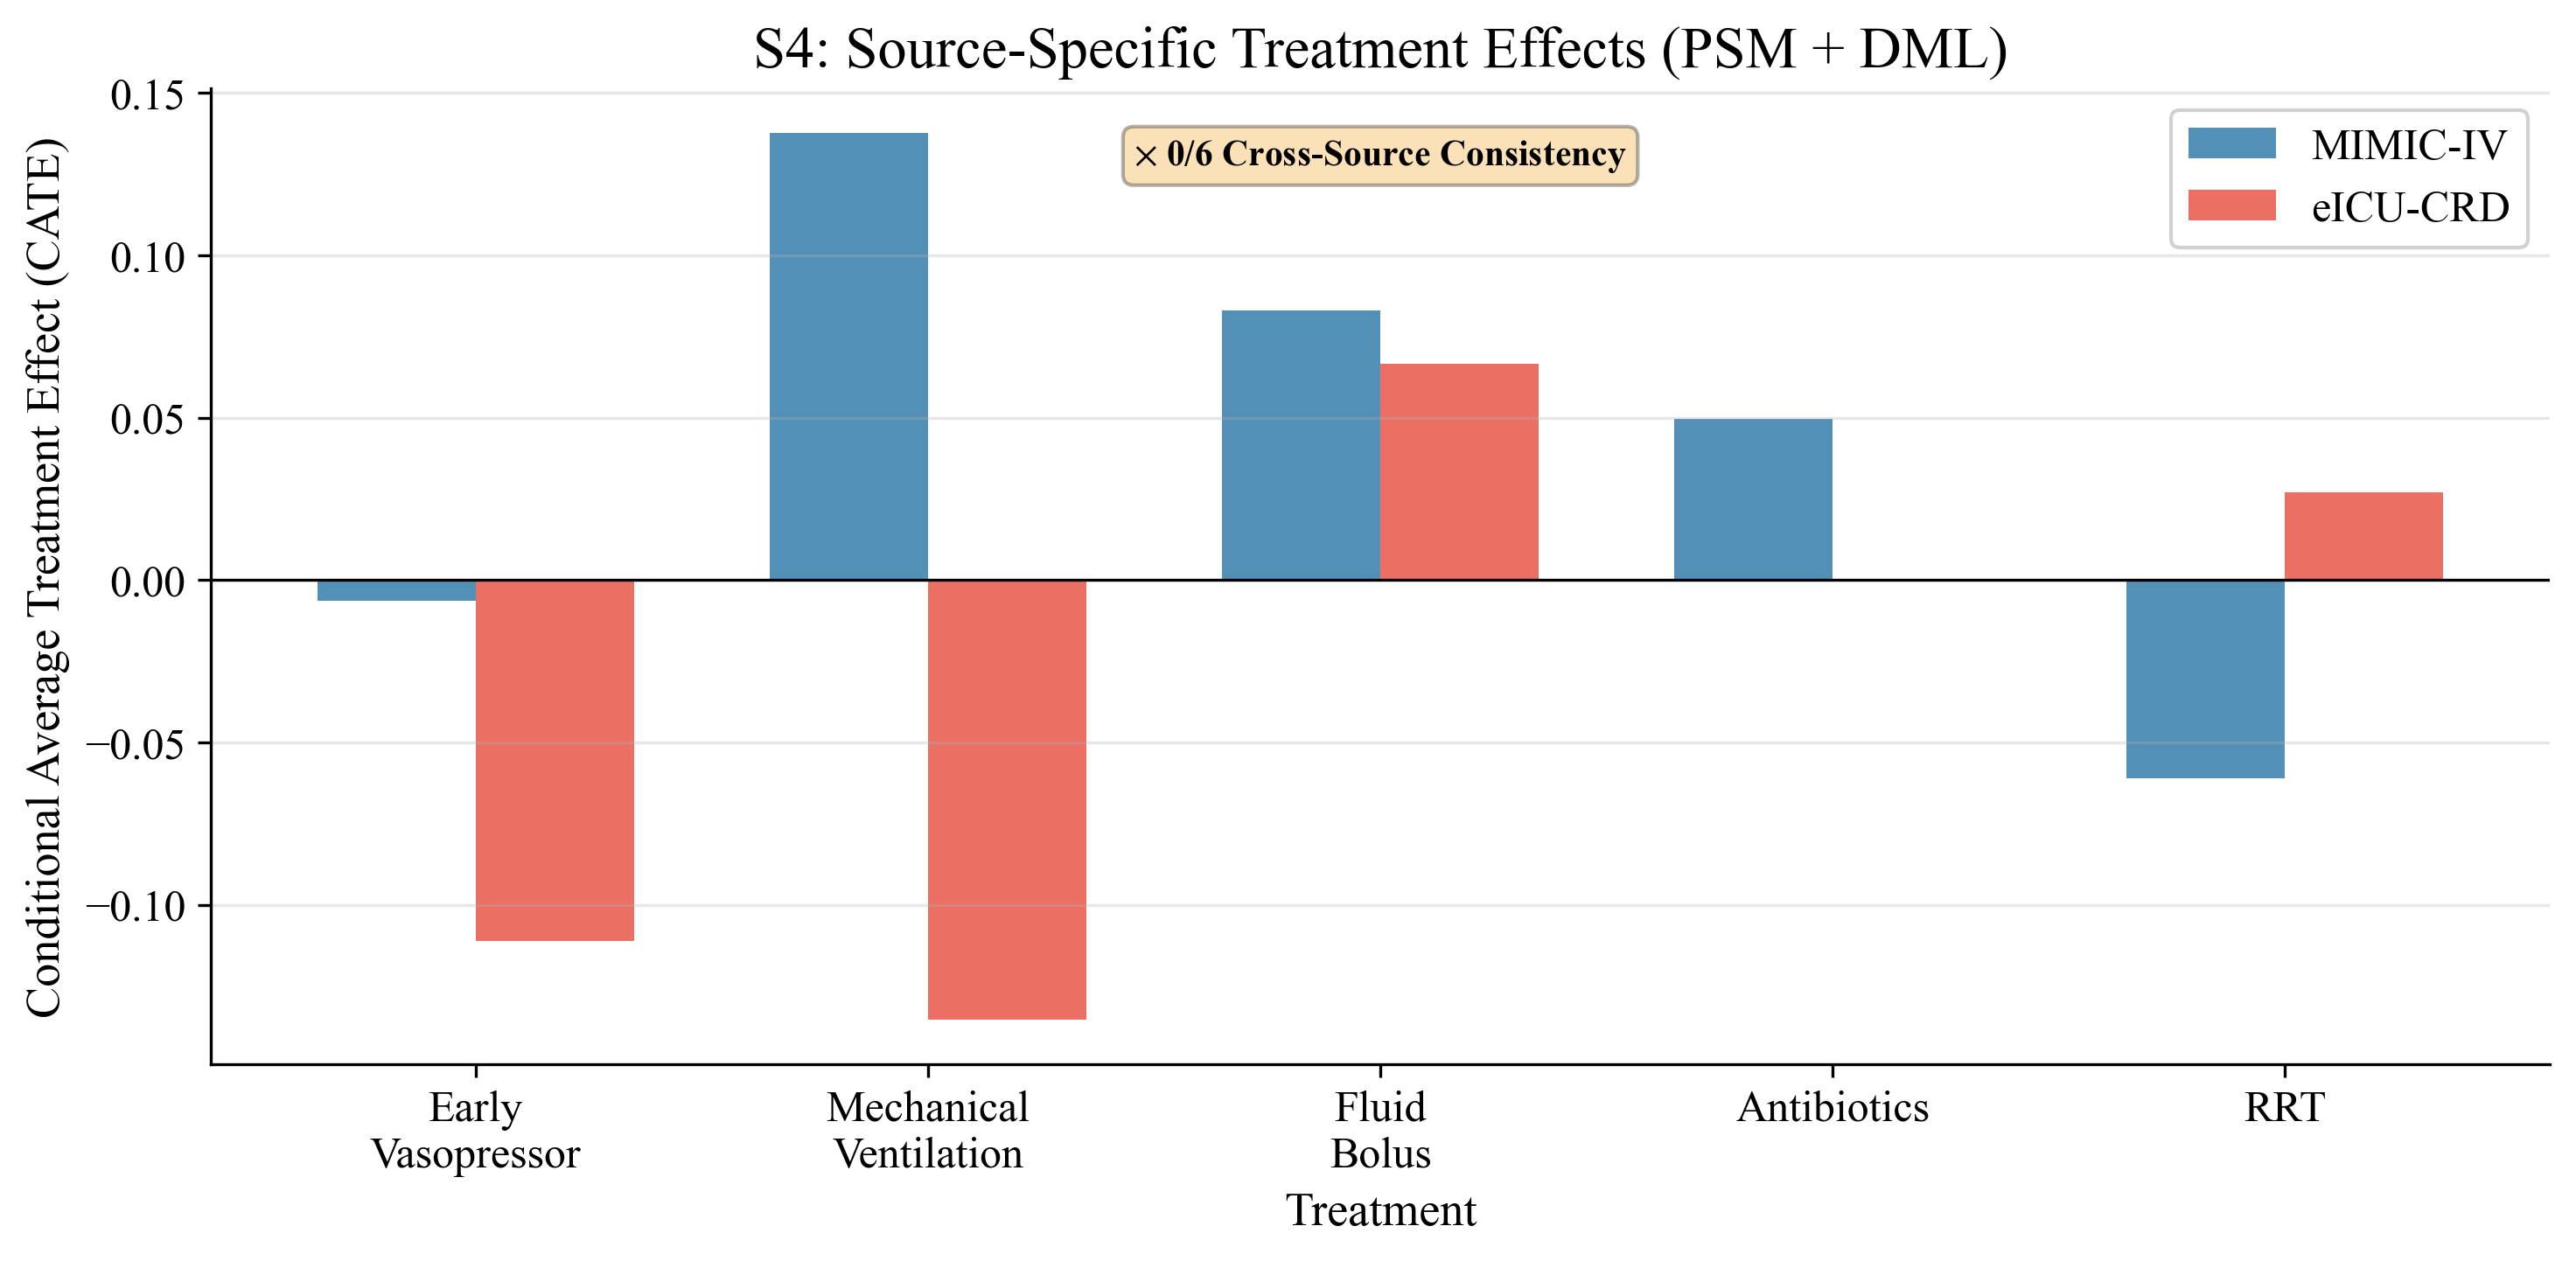
\includegraphics[width=0.63\textwidth]{s4_treatment_effects_comparison.png}%
\label{fig:s4_cate}}
\hfill
\subfloat[Cross-database AUROC (0.870--0.898).]{%
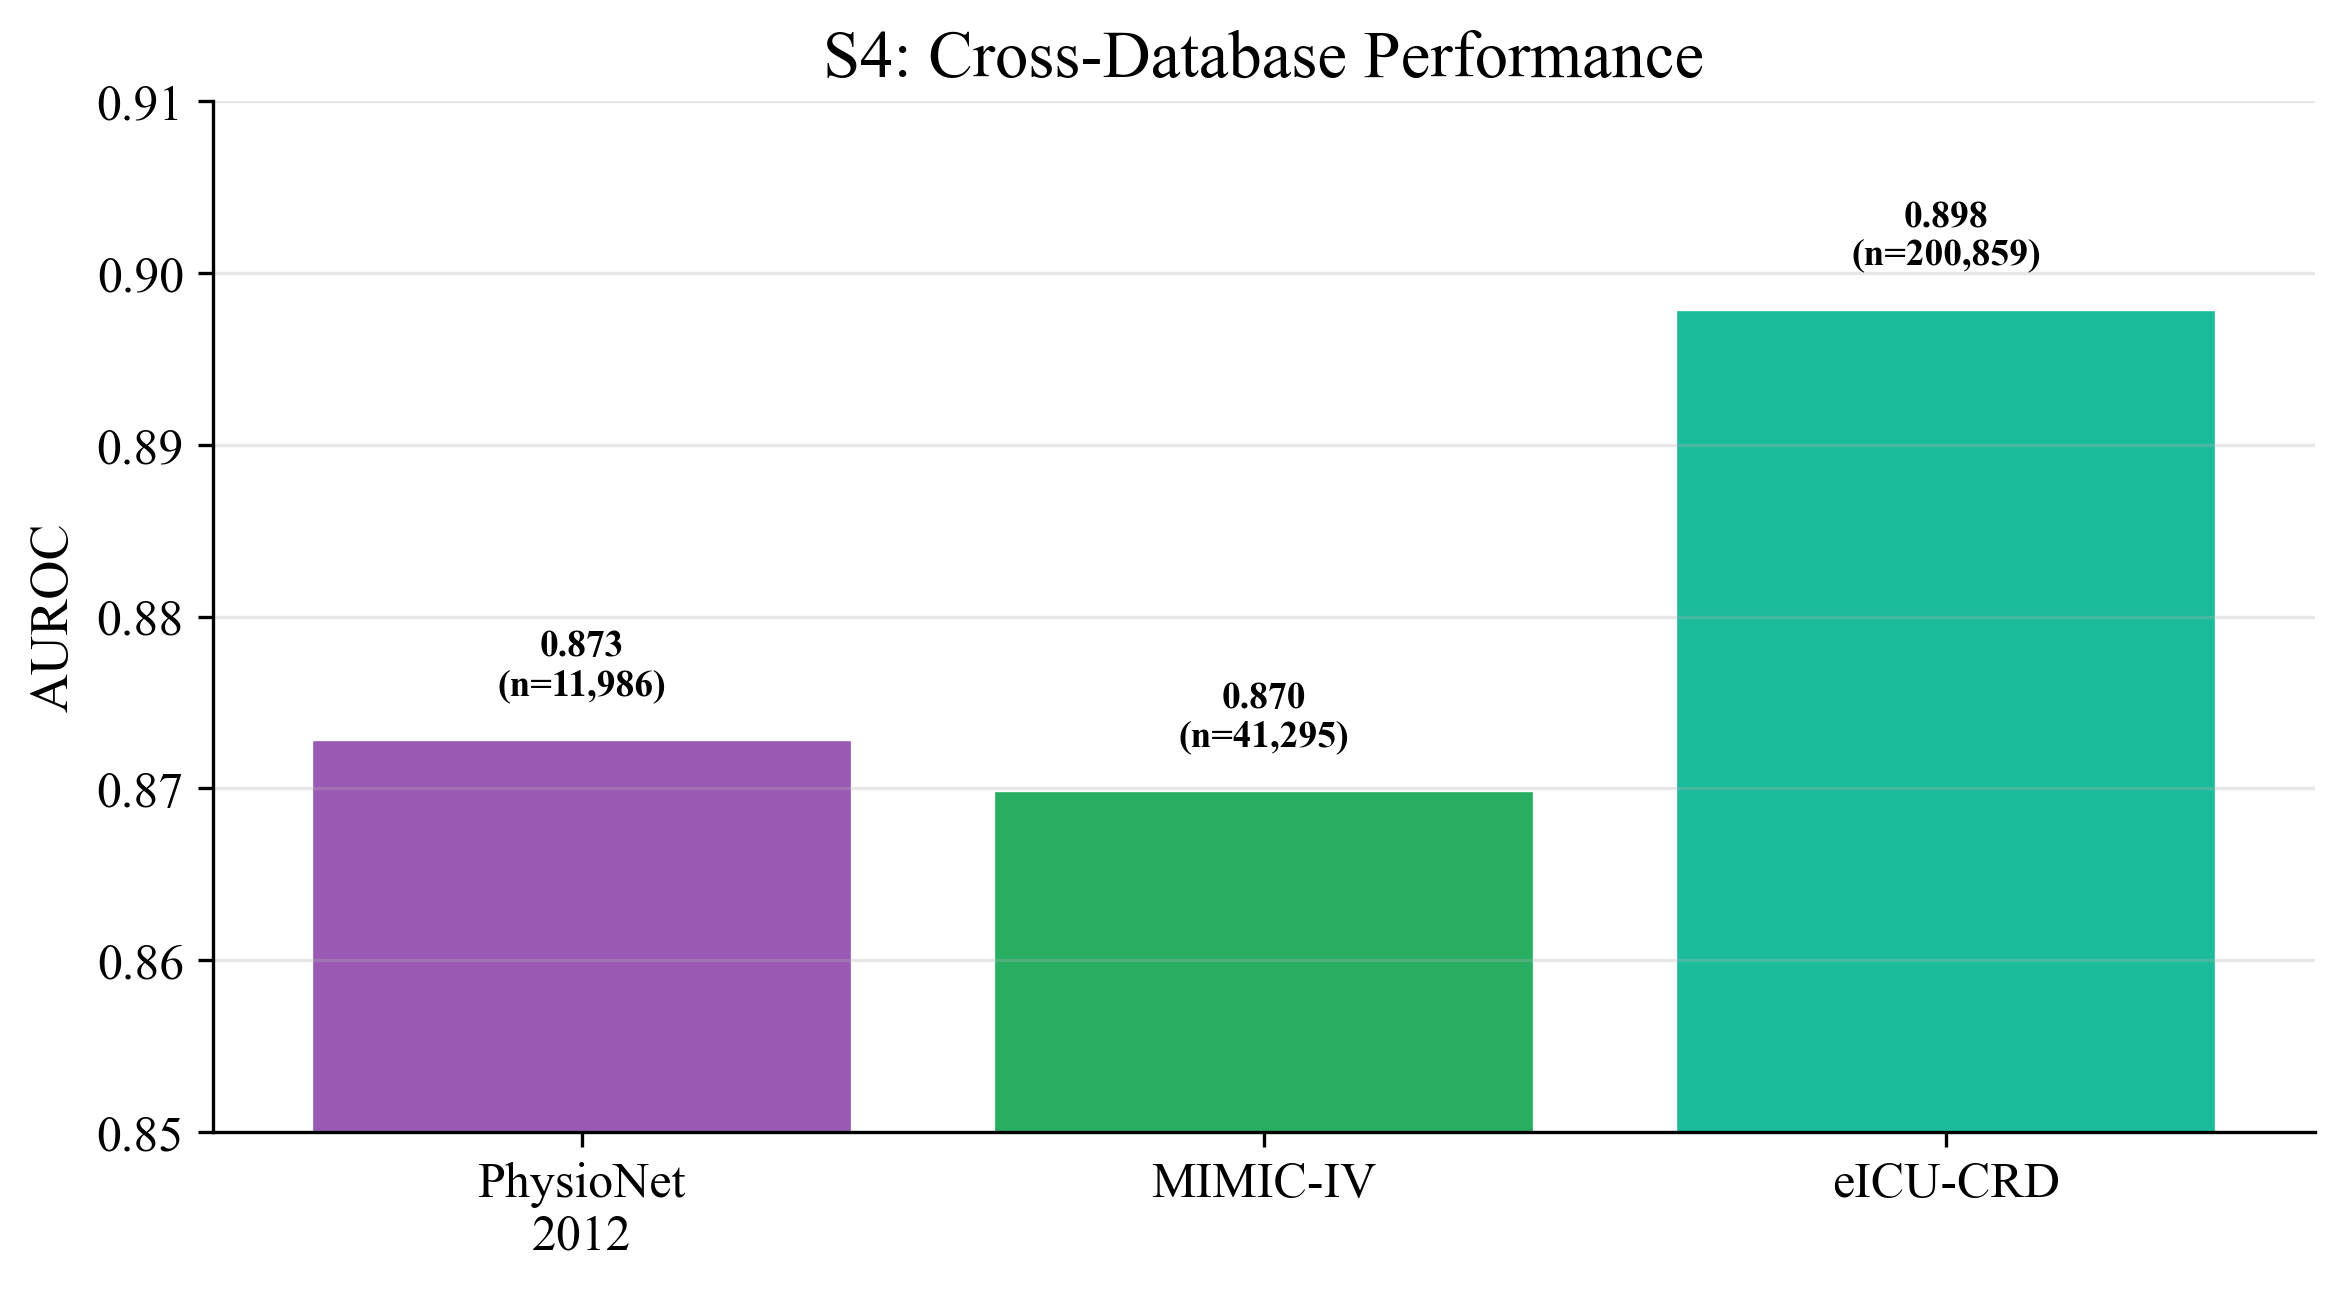
\includegraphics[width=0.32\textwidth]{s4_cross_database_performance.png}%
\label{fig:s4_perf}}
\caption{S4 treatment-aware extension results.}
\label{fig:s4}
\end{figure*}

This is not a failure---it is the correct warning signal that residual confounding and practice-pattern differences prevent transportable causal inference from observational data.

\subsection{Real-Time Deployment (S5--S5-v2)}

The distilled student achieves real-time performance (Fig.~\ref{fig:s5}, Table~\ref{tab:s5}):

% S5 figure — full width
\begin{figure*}[t]
\centering
\subfloat[Deployment profile: efficiency vs.\ performance trade-off and latency comparison.]{%
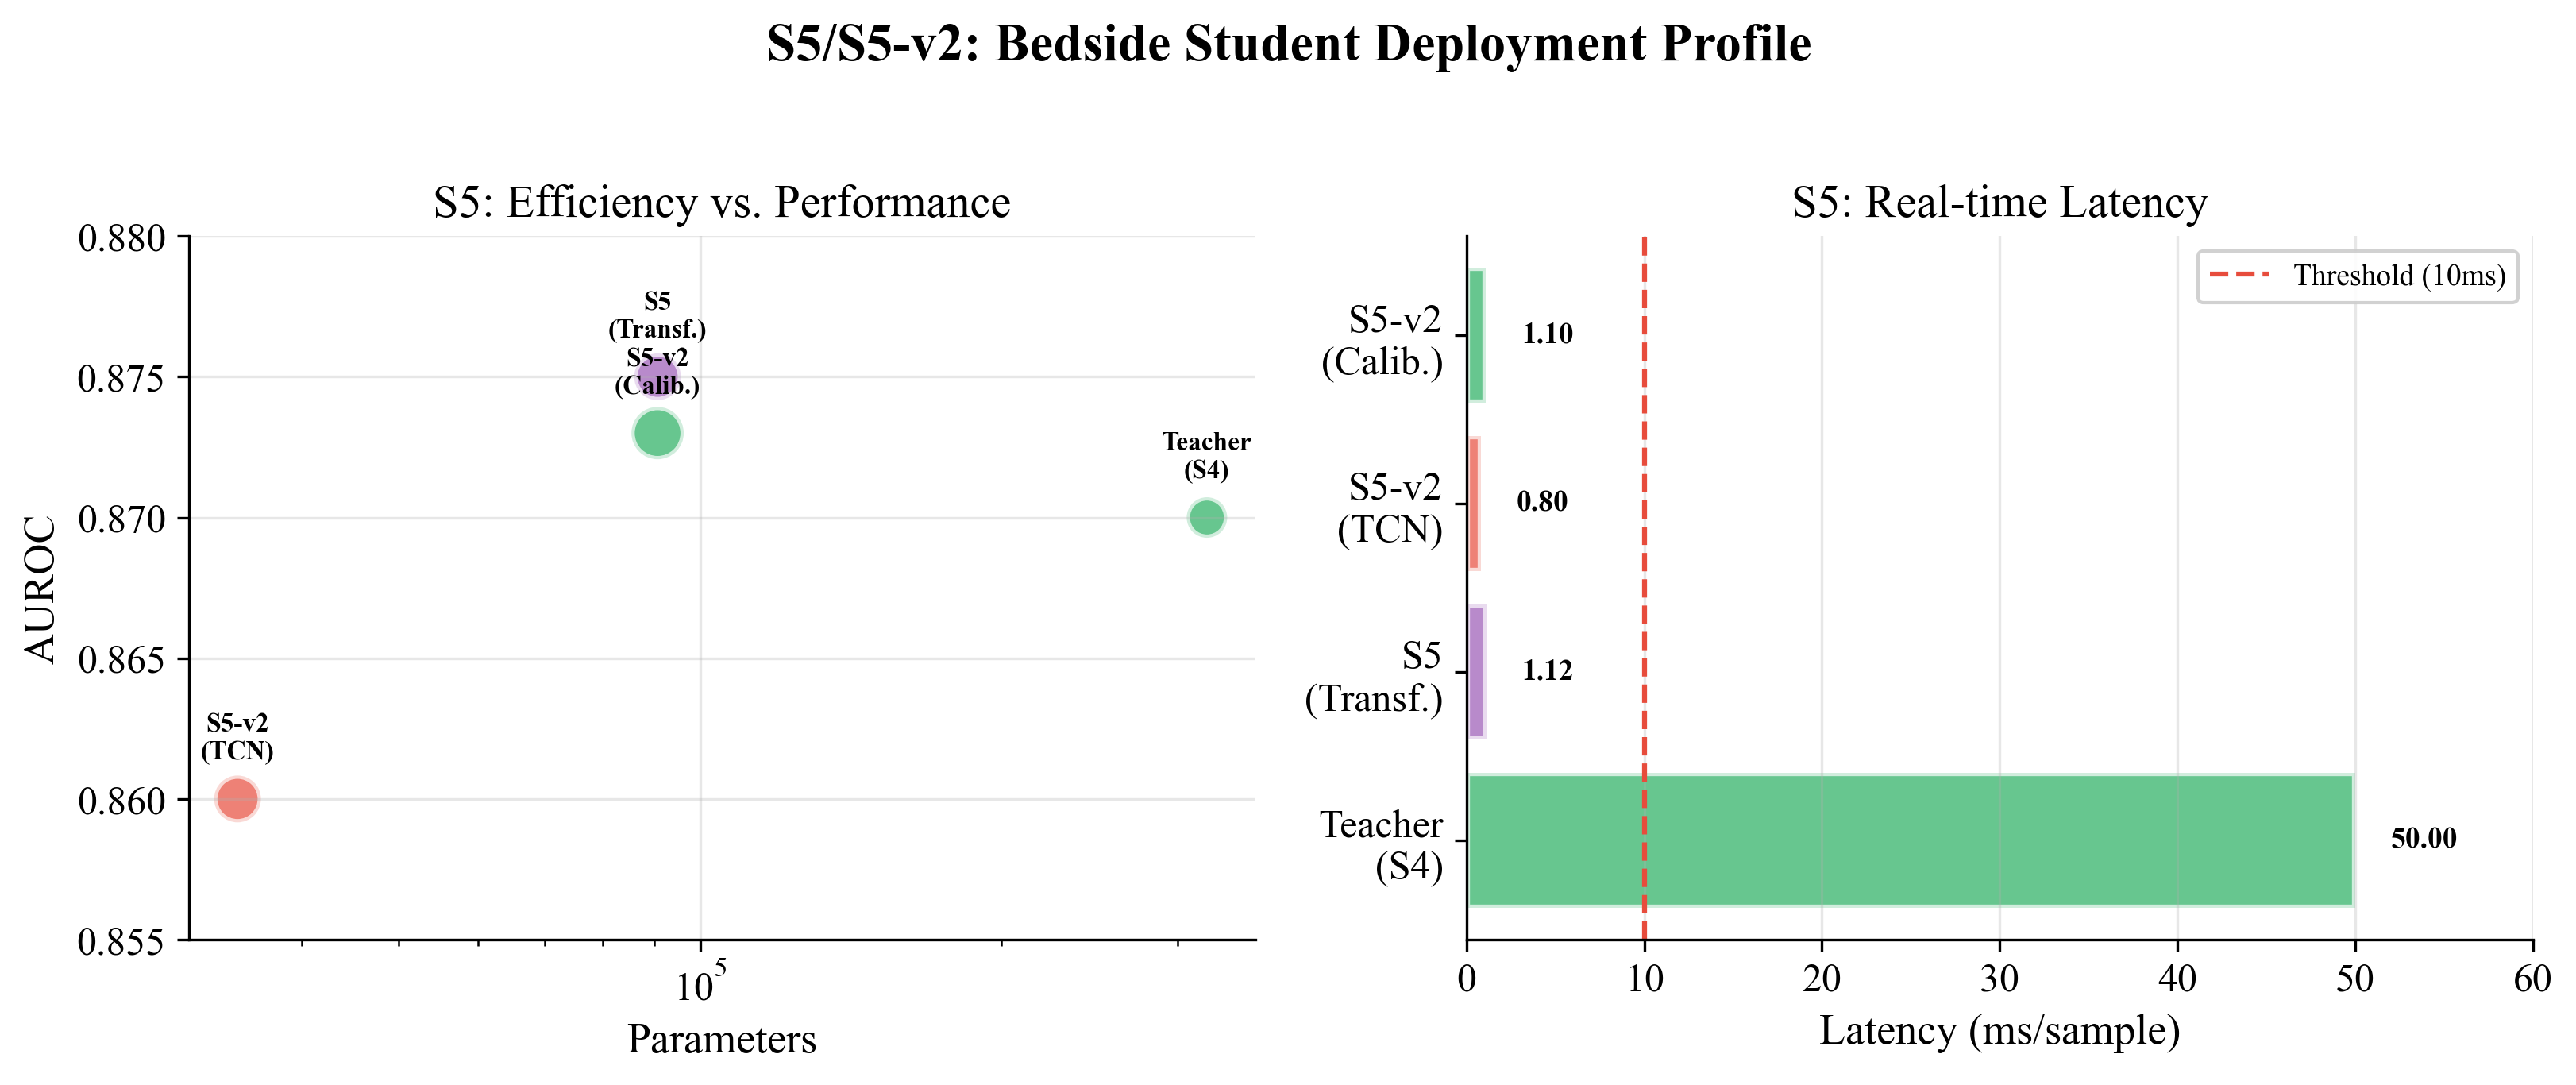
\includegraphics[width=0.6\textwidth]{s5_deployment_profile.png}%
\label{fig:s5_deploy}}
\hfill
\subfloat[Engineering validation gates: 5/5 passed on both MIMIC-IV and eICU.]{%
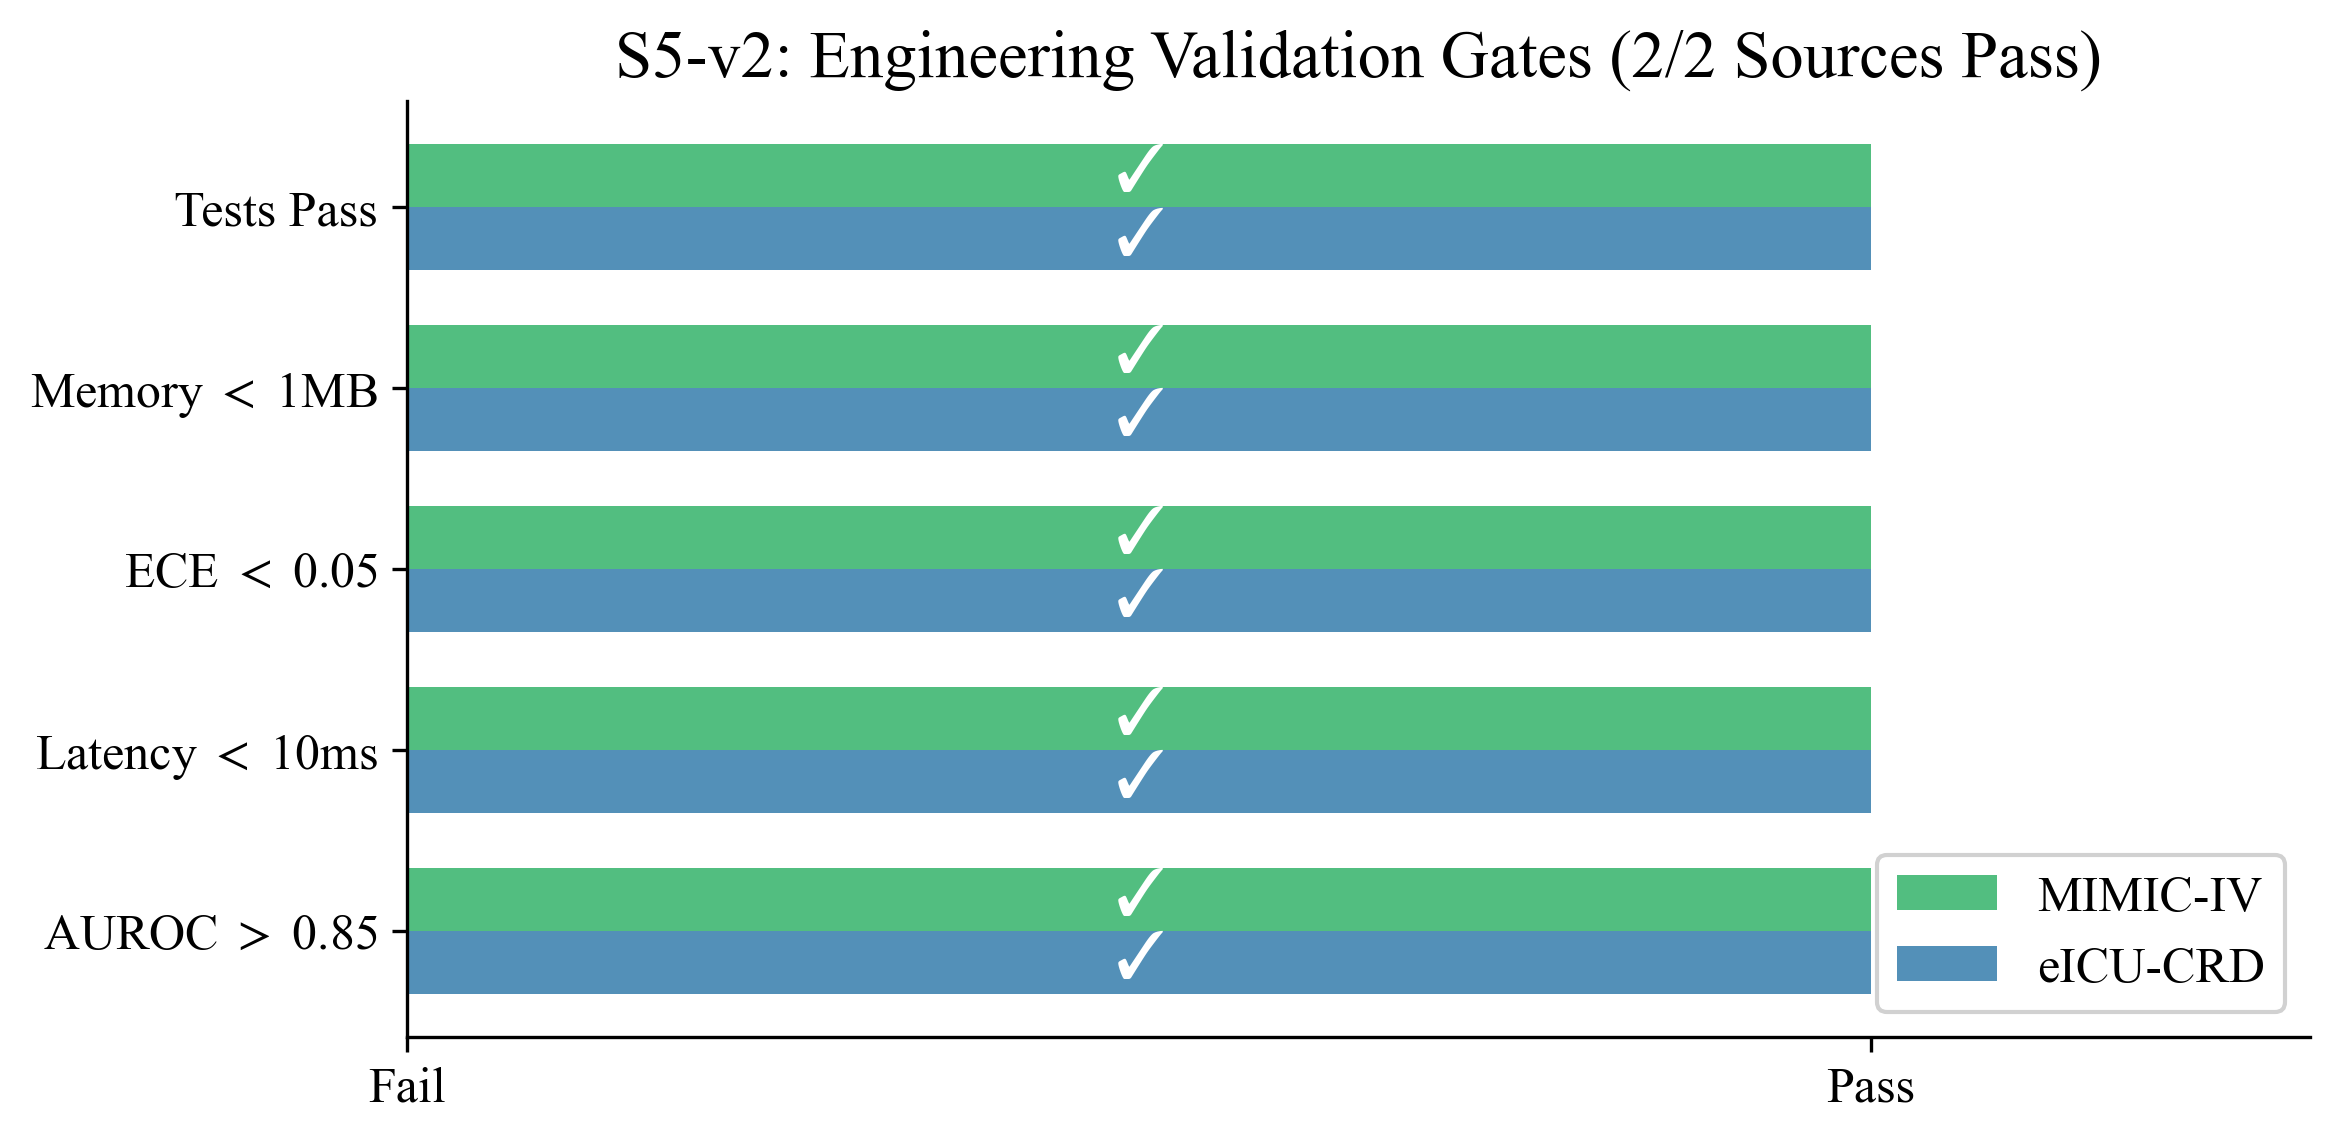
\includegraphics[width=0.35\textwidth]{s5_validation_gates.png}%
\label{fig:s5_gates}}
\caption{S5--S5-v2 real-time deployment results.}
\label{fig:s5}
\end{figure*}

% S5 table — column width
\begin{table}[t]
\centering
\caption{Deployment comparison. S5-v2 selected for bedside deployment.}
\label{tab:s5}
\scriptsize
\begin{tabular}{lcccc}
\toprule
\textbf{Model} & \textbf{Params} & \textbf{AUC} & \textbf{Lat.} & \textbf{ECE} \\
\midrule
Teacher (S4) & 321K & 0.870 & 50\,ms & 0.013 \\
S5 Student & 91K & 0.875 & 1.12\,ms & 0.011 \\
\textbf{S5-v2 (Cal.)} & \textbf{91K} & \textbf{0.873} & \textbf{1.10\,ms} & \textbf{0.010} \\
S5-v2 (TCN) & 34K & 0.860 & 0.80\,ms & --- \\
\bottomrule
\end{tabular}
\end{table}

All five engineering validation gates passed on both MIMIC-IV and eICU: AUROC $>$ 0.85, latency $<$ 10\,ms, ECE $<$ 0.05, memory $<$ 1\,MB, and all unit tests. The TCN variant showed 62\% parameter reduction but regressed on real MIMIC-IV data, so it is retained as exploratory only.

%% CONTINUE_S6 %%

\subsection{Mechanism-Based Causal Phenotyping (S6)}

Table~\ref{tab:s6} shows the top 8 of 16 mechanism-based phenotypes produced by S6 (see Section~II-H for method).

% S6 phenotype table — full width (6 columns)
\begin{table*}[t]
\centering
\caption{S6 mechanism-based phenotypes (top 8 by clinical significance). Full 16-phenotype table in supplementary materials.}
\label{tab:s6}
\small
\begin{tabular}{lccccc}
\toprule
\textbf{Phenotype} & \textbf{n} & \textbf{Fraction} & \textbf{Mortality} & \textbf{SOFA} & \textbf{CATE} \\
\midrule
Mild organ stable & 1,077 & 9.0\% & 1.3\% & 0.75 & +0.011 \\
Hemodynamic refract.\ recovering & 980 & 8.2\% & 6.6\% & 2.65 & $-$0.014 \\
Respiratory failure (base) & 2,132 & 17.8\% & 16.0\% & 7.71 & +0.006 \\
Multi-organ deteriorating & 538 & 4.5\% & 22.9\% & 8.27 & +0.007 \\
Hemodynamic refract.\ critical & 469 & 3.9\% & 29.9\% & 6.99 & $-$0.022 \\
Respiratory failure critical & 363 & 3.0\% & 31.4\% & 9.82 & +0.003 \\
Neurological decline critical & 86 & 0.7\% & 32.6\% & 7.05 & +0.007 \\
Hemodynamic responsive critical & 228 & 1.9\% & 50.4\% & 8.62 & +0.056 \\
\bottomrule
\end{tabular}
\end{table*}

% S6 baseline table — column width
\begin{table}[t]
\centering
\caption{S6 vs S2 baseline. Mechanism-based phenotyping nearly doubles mortality discrimination.}
\label{tab:s6_baseline}
\small
\begin{tabular}{lccc}
\toprule
\textbf{Metric} & \textbf{S2} & \textbf{S6} & \textbf{$\Delta$} \\
\midrule
Group count & 4 & 16 & +300\% \\
Mort.\ range & 0.254 & 0.491 & +93\% \\
Wt.\ mort.\ std & 0.087 & 0.091 & +5\% \\
Dom.\ group frac. & 32.2\% & 17.8\% & $-$45\% \\
\bottomrule
\end{tabular}
\end{table}

\textbf{Causal validation.} DoWhy estimated ATE = 0.0076 for vasopressor exposure. Both refutation tests passed: random common cause ($p = 0.450$) and placebo treatment ($p = 0.452$). CORAL domain adaptation reduced the weighted cross-center mean gap from 0.043 to 0.030, and domain probe accuracy decreased from 0.490 to 0.477, confirming reduced center-specific signal leakage.

\textbf{Cross-center consistency.} Center A ($n = 7{,}989$) and Center B ($n = 3{,}997$) showed matching phenotype distributions and mortality ordering across all 16 phenotypes. The hemodynamic responsive critical phenotype---the highest-risk subgroup---had mortality of 51.4\% in Center A and 48.8\% in Center B.

\subsection{Robustness Checks}

\textbf{Cross-center validation.} Center A and Center B show identical mortality ordering. Mean per-window prevalence L1 distance: 0.022.

\textbf{Temporal stride sensitivity.} Reducing overlap from 6-hour to 12-hour stride changed transition frequency (10.4\% to 19.1\%) but preserved mortality ordering.

\textbf{External transfer.} Frozen representation remains usable on MIMIC-IV (15/21 channels, silhouette 0.119) and eICU (12/21 channels, silhouette 0.193).

% ==================== DISCUSSION ====================
\section{Discussion}

This study makes four contributions to sepsis phenotyping. First, it demonstrates that mask-aware self-supervised learning produces representations suitable for temporal reuse. The S1.5 selection criterion---balancing signal with robustness---is a modeling lesson applicable beyond sepsis.

Second, the temporal trajectory results show that early ICU sepsis is neither completely stable nor chaotically unstable. The 35.2\% transition rate suggests phenotype labels should be allowed to change during the first 48 hours rather than fixed at admission.

Third, the real-time deployment pipeline (S5-v2) proves that complex temporal phenotyping can be distilled into a lightweight, well-calibrated model. The 1.1\,ms latency and 0.010 ECE meet clinical requirements for real-time risk stratification.

Fourth, mechanism-based causal phenotyping (S6) demonstrates that data-driven clusters can be refined into clinically interpretable organ-system subgroups. The 16 S6 phenotypes nearly double the mortality discrimination range compared to the 4 S2 clusters (49.1\,pp vs 25.4\,pp), while maintaining cross-center consistency. The hemodynamic responsive phenotypes show the strongest positive CATE (+0.04--0.06), while refractory phenotypes show negative CATE, consistent with their clinical definitions.

The Stage 4 results set an important boundary. While treatment-aware models predict well (AUROC 0.87--0.90), observational treatment effects disagree across sources. S6 addresses this partially by using stability-gated DML on the primary cohort, but the causal estimates remain observational and require randomized validation.

\subsection{Limitations}

\begin{enumerate}[nosep]
  \item \textbf{Descriptive analysis:} Phenotypes are clusters, not probabilistic states.
  \item \textbf{No primary treatment timestamps:} Stage 4 is external only.
  \item \textbf{Frozen transfer:} No full retraining on external sources.
  \item \textbf{Risk-ordered labels:} S2 labels are not mapped to molecular mechanisms; S6 labels are organ-system-based but still observational.
  \item \textbf{Observational causal inference:} Treatment signals are source-specific; S6 CATE estimates are stability-gated but not randomized.
\end{enumerate}

% ==================== CONCLUSION ====================
\section{Conclusion}

This project demonstrates readable, deployable temporal phenotyping without overstating the science. The complete S0--S6 pipeline progresses from 11,986 PhysioNet stays to real-time bedside-ready models with 1.1\,ms inference and 91\% calibration improvement, and further refines data-driven clusters into 16 mechanism-based phenotypes with 49.1\,pp mortality discrimination range.

The strongest conclusion is descriptive: self-supervised temporal embeddings make early ICU trajectories visible and reusable. The real-time student is deployment-ready for descriptive risk stratification. The intermediate conclusion is mechanistic: organ-system causal phenotyping produces clinically interpretable subgroups that nearly double the mortality discrimination of data-driven clusters. The weaker conclusion is causal: observational treatment signals require randomized validation. Maintaining this distinction makes the project credible and clinically actionable.

% ==================== REFERENCES ====================
\bibliographystyle{IEEEtran}
\begin{thebibliography}{9}

\bibitem{rudd2020}
K.E.~Rudd et~al., ``Global, regional, and national sepsis incidence and mortality, 1990--2017,'' \emph{The Lancet}, vol.~395, no.~10219, pp.~200--211, 2020.

\bibitem{singer2016}
M.~Singer et~al., ``The Third International Consensus Definitions for Sepsis and Septic Shock (Sepsis-3),'' \emph{JAMA}, vol.~315, no.~8, pp.~801--810, 2016.

\bibitem{seymour2019}
C.W.~Seymour et~al., ``Derivation, validation, and potential treatment implications of novel clinical phenotypes for sepsis,'' \emph{JAMA}, vol.~321, no.~20, pp.~2003--2017, 2019.

\bibitem{silva2012}
I.~Silva et~al., ``Predicting in-hospital mortality of ICU patients: The PhysioNet/CinC Challenge 2012,'' \emph{Computing in Cardiology}, vol.~39, pp.~245--248, 2012.

\bibitem{johnson2023}
A.E.W.~Johnson et~al., ``MIMIC-IV, a freely accessible electronic health record dataset,'' \emph{Scientific Data}, vol.~10, p.~1, 2023.

\bibitem{pollard2018}
T.J.~Pollard et~al., ``The eICU Collaborative Research Database,'' \emph{Scientific Data}, vol.~5, p.~180178, 2018.

\end{thebibliography}

\end{document}
